\chapter{Literature Review}\label{ch:litreview}

This literature review seeks to satisfy two primary purposes. The first is to
present an overview and analysis of the current landscape of nuclear fuel cycle
simulation in \S \ref{sec:simulators}. Such a discussion provides the general
backdrop for the proposal laid out in \S \ref{sec:agent-interaction} as well as
the remaining research proposal. The second is to provide an overview of the
tools and algorithms used to formulate and solve the proposed problems in \S
\ref{sec:gfctp} and \S \ref{sec:rap}. This work crosses multiple disciplines,
namely nuclear engineering and systems engineering, thus discussions of linear
programming in \S \ref{sec:lp} and integer programming in \S \ref{sec:ip} seek
to provide a minimal and reasonable set of information regarding mathematical
programming to lay a basic foundation for readers unaccustomed to the
discipline.

\section{State of the Art of Fuel Cycle Simulation}\label{sec:simulators}
A number of current fuel cycle simulators are reviewed in this section with a
keen focus of simulation-developer related design aspects. There are broadly two
main categories that simulation developers must address: how simulation entities
enter a given simulation and how simulation entities interact, or are connected,
in a simulation. The former varies by each simulator, whereas the latter is
handled by proprietary system dynamics software in most cases. Peripheral
concerns are also addressed, namely simulation input/output and the associated
coding platform(s). Because all current fuel cycle simulators are effectively
closed source, any knowledge of their inner workings must be gleaned from the
available literature published by their respective development
teams. Additionally, summary information can be gathered from the MIT
benchmarking exercise \cite{guerin_benchmark_2009}, because the sections
corresponding to each simulator were written by the simulator developers. From a
developers perspective, assumptions are made when the literature does not
provide a clear explanation of a given design decision, but such assumptions are
expressly noted.


\subsection{COSI}\label{sec:cosi}
Commelini-Sicart (COSI) is a fuel cycle simulation code developed by the French
Commissariat \`{a} l'\'{e}nergie atomique (CEA), written in the Java programming
language. Accordingly, it can be classified as an object oriented simulator. The
stated goal of COSI is to model the amount and isotopics of material at each
stage in the fuel cycle, explicitly modeling reactor parks and their supporting
facilities (i.e., enrichment, separations, and fuel fabrication) in order to
study transition scenarios at a high level of isotopic and physical
fidelity. Its origins date to 1991, and it has been updated with relative
frequency since 2005 \cite{boucher_cosi_2005,boucher_cosi:_2006,meyer_new_2009,
coquelet-pascal_validation_2011}.

The main user input for a COSI simulation is period to be simulated and the
commissioning and decommissioning date for each type of reactor in the
simulation. It does not deploy reactors based on any sort of algorithmic
model. Users are also allowed to choose the processing order of spent fuel
(e.g. first in/first out, as a function of burnup, as a function of Pu-241
content, etc.).

In general, reactors are assumed to be fueled with material whose makeup
corresponds to an equilibrium cycle. For each type of reactor, a single fuel
type is assumed to be used. COSI usese a family of methods for determining input
fuel isotopics, the aggregate name of which is an ``Equivalence Model''. The
term refers to an ``equivalent fraction'' of fissile isotopes in fabricated fuel
comprised of fissile and fertile isotopes given a target fertile fraction and
available isotopics of separated fuel. In the simplest case, i.e., for enriched
uranium oxide (UOX) fuel, the model is simply a predefined enrichment.
Similarly, for mixed plutonium-uranium oxide (MOX) fuel for use in thermal
reactors, the equivalence model is simply a predefined plutonium content. It is
not clear, however, if the plutonium content is in total mass or mass of a
specific plutonium isotope \cite{meyer_new_2009,
coquelet-pascal_validation_2011}. Further, I assume that a similar equivalence
model is used for any other thermal reactor fuel. Specifically, this set of
models requires a class fertile of material (e.g. depleted uranium, recycled
uranium, natural uranium) and a class of fissile material (e.g. plutonium,
transuranics), and a predefined ratio of the two. It is unclear how many degrees
of freedom a user has in defining these parameters for each reactor. In any
case, UOX is a special case of the equivalence model, because it has no
restrictions on its fabrication, i.e., COSI does not allow natural uranium
availability to be a constraining parameter in a simulation.

In order to determine the input isotopics for fast reactors, COSI uses an old
technique developed by Baker and Ross \cite{baker_comparison_1963}. In fact,
this is where the original notion of an ``equivalence method'' originates. The
core premise of this method is that a fast reactor at equilibrium is ideally
loaded with Pu-239 and U-238. Accordingly, deviations from this ideal
composition must be accounted for. Baker and Ross describe an equilibrium
analysis in which ``for a system initially just critical, the reactivity is
maintained zero'', which is ``justified by perturbation theory''. They describe
this condition mathematically as

\begin{equation*}
\sum_{i \in I} \left( \nu_{i} \sigma_{f,i} - \sigma_{a,i} \right) N_i = c,
\end{equation*}

where $c$ is a constant, and for a given isotope $i$ in the set of heavy fuel
elemental isotopes, $I$, $N_i$ is its average number density, $\nu_{i}$ is the
average number of neutrons resulting from its fission, $\sigma_{f,i}$ is its
microscopic fission cross section, and $\sigma_{a,i}$ is its microscopic
absorption cross section. For convenience, let us define the collection of
isotopic parameters as

\begin{equation*}
x_i = nu_{i} \sigma_{f,i} - \sigma_{a,i}.
\end{equation*}

Baker and Ross then note that one can approximate the critical mass of plutonium
required for a given mixture of plutonium isotopes using an isotopic worth,
$w_i$, that is a function of its deviation from pure plutonium-239,

\begin{equation*}
w_i = \frac{x_i - x_{^{238}U}}
           {x_{^{239}Pu} - x_{^{238}U}}.
\end{equation*}

Then, for any combination that makes a core critical, the following holds

\begin{equation*}
\sum_{i \in I} m_i w_i = c,
\end{equation*}

where $m_i$ is the mass of isotope $i$.

The COSI team adapts this approximation method for its use in order to determine
the fuel composition of fast reactors. Given an ideal plutonium-239 enrichment,
$E_0$, and for each isotope in a set of fertile and fissile isotopes, $I_{Fe}$
and $I_{Fi}$, respectively, the isotopic neutronic weights, $w_i$, and available
isotopic weight fractions, $\xi_i$, one can compute an equivalent fissile
isotope enrichment, $E$.

\begin{equation*}
E = \frac{E_0 - \sum_{i \in I_{Fe}} \xi_i w_i}
         {\sum_{i \in I_{Fi}} \xi_i w_i - \sum_{i \in I_{Fe}} \xi_i w_i}
\end{equation*}

This perturbed fissile enrichment is then used to determine the amount of
material to take from available fissile stockpiles and the amount of material to
take from available fertile stockpiles, i.e., $1 - E_0$.

It is important to note that the resulting isotopics for either thermal or fast
reactor fuel is a function of the user-defined reprocessing order. The
equivalence model simply determines the quantity of fertile and fissile material
to extract from the available stockpiles. Granted, the equivalence models
are \textit{informed} by the isotopics of those stockpiles, but they are
considered constants in the calculation. Further, the level of fidelity of
modeling of the separations and fabrications facilities are not explicitly
stated. In the COSI literature, the authors refer to batches of material, but
never define explicitly what a batch is. 


\subsection{CAFCA}\label{sec:cafca}
The Code for Advanced Fuel Cycles Assessment - System Dynamics (CAFCA-SD) is
developed at the Massachusetts Institute of Technology (MIT). Originally
developed in MATLAB, it is currently an application written in the commercial
software VENSIM \cite{vensim_2010_ventana} ``with potential interactions with
C++ programs'' \cite{guerin_benchmark_2009}. CAFCA-SD has gone through a number
of developmental iterations. It originally was designed to analyze transuranic
(TRU) recycling in fertile/fertile-free and actinide-burning reactors. It was
then extended to incorporate fast, self-sustaining reactors (i.e., with a
conversion ratio of unity) and to allow constraints on reprocessing facility
capacity factors. The third update allowed for isotope tracking and the decay of
isotopes, however, the CAFCA literature states that it does not incorporate the
use of decay and claims such capability does not greatly affect results
\cite{guerin_impact_2009,guerin_benchmark_2009}. The final iteration
improvements include the ability to model fuels such as mixed-oxide fuels (MOX)
and ``high burnup fuel in thermal reactors'', fast reactors with conversion
ratios other than unity, and the use of multiple fuel technologies that require
recycling in the same scenario (for example, having MOX fuel being recycled
multiple times). Time steps in CAFCA-SD occur every 1.5
months \cite{guerin_impact_2009}, at which point discrete events are executed to
change the system state that depend on the current system state.

The main user-provided parameters for a simulation are the power demand for
nuclear reactors, which is modeled as an exponential cuver, and the fraction of
TRU or minor actinides (MA) to provide for each reactor technology. TRU set
aside for each technology is essentially modeled as a different fuel type
(e.g., TRU for MOX and TRU for Fast Reactors). The simulation framework uses
these fractions to determine the total number of reactors that can be fuel for
each type of reactor. Users also set a number of other parameters, such as
reactor power and other reactor characteristics, but the above two parameter
categories govern the actual course of the simulation with respect to building
reactors and determining material flows. The forcing function for the
simulation, is the availability of recycled fuel. In other words, as one of
CAFCA's basic simulation assumptions, the inventory of used light water reactor
(LWR) fuel is minimized. Thus the number of reactors using this recycled fuel is
maximized against this constraint, according to the user-defined fuel technology
preference fractions. 

As previously stated, CAFCA-SD determines the evolution of system states using
system dynamics. It should be noted that the CAFCA team states explicitly that
their model should be used for large scoping studies \cite{guerin_impact_2009},
which informs their simulation methodology and inherent assumptions. Their
overall system model is comprised of coupled single-input, single-output
structure-policy diagrams. Each structure-policy diagram is composed of a
system-structure substructure and a policy-structure substructure, which defines
decision rules for the diagram. The beginning of a time step invokes the
application of decision rules which changes the state of the system. The new
state is then updated in the system structure, which informs new decision
rules. Each diagram is connected to others via their input or output. Examples
of such diagrams are: the LWRs structure-policy diagram, the front-end
structure-policy diagram, and the back-end structure-policy diagram. Further,
there are diagrams for each reactor fuel type that requires new technologies
(e.g., MOX, ABR).

In general, CAFCA does not model individual
facilities \cite{guerin_impact_2009}. Furthermore, it only explicitly models
reactors and reprocessing facilities. The remaining entities, which are
conceptually connected to the instantiated entities via markets, are assumed to
belong to completely elastic markets, i.e., demand is always met. Instead of
modeling individual facilities, it models rate changes of fleets of facilities
and monitors the status of those fleets (i.e., how many should currently be in
operation). This methodology is perhaps not intuitively obvious, so let me
briefly follow a similar overview of such a process as provided in CAFCA's
original methodology report \cite{busquim_e_silva_system_2008}. First, though, a
note on their notation; CAFCA's methodology denotes many system variables as a
function of time for each class (fleet) of reactors, which are described in
Table \ref{tbl:cafca-rxtr-vars}.

Before wading too deep into CAFCA's methodology formulation, let me take a
moment to reflect on the variables in Table \ref{tbl:cafca-rxtr-vars}. The
actual definition of the various rates and stocks described therein depend on
the type of reactor they are describing. Any reactor that is fueled in some part
by material that is output from reprocessing facilities has the same general
form, which incorporates the respective user-defined percentages previously
discussed. This makes sense, of course, because CAFCA's simulation methodology
only allows advanced reactors to be built if they can be fueled for their entire
lifetimes. Accordingly, their building rate depends on the availability of
recycled fuel. Reactors that use non-recycled fuel, i.e., light water reactors
(LWRs), have different formulations. There is no restriction on their building
based on fuel availability (their input fuel markets are assumed totally liquid
as stated above), and so their rate and state values which are informed by the
number of recycle-fueled reactors in operation. In other words, LWRs ``fill the
holes'' in energy demand left by fast reactors that can't otherwise make them up
due to lack of input fuel. The cycle is connected because LWRs provide the
source of fast reactor fuel.

%%% 
\begin{table} [h!]
\centering
\begin{tabularx}{\textwidth-20pt}{|c|X|} % line wraps second column if too long
\hline
Variable    & Description \\
\hline
$P_r$            & the power rating for reactors of fleet $r$ \\
$CF_r$           & the capacity factor rating for reactors of fleet $r$ \\
$F^r_{Est}(t)$   & the forecasted fleet requirements for the fleet of $r$ at time $t$  \\
$F_r(t)$         & the actual fleet requirements for the fleet of $r$ at time $t$  \\
$ADJ_r(t)$       & the adjustment for the fleet of $r$ at time $t$  \\
$\tau_r(t)$      & the fleet adjustment time for the fleet of $r$ at time $t$  \\
$R^r_{CO}(t)$    & the construction order rate for the fleet of $r$ at time $t$  \\
$R^r_{FO}(t)$    & the fulfilled order rate for the fleet of $r$ at time $t$  \\
$R^r_{FO}(t)$    & the fulfilled order rate for the fleet of $r$ at time $t$  \\
$R^r_{Frac}(t)$  & the fractional order rate for the fleet of $r$ at time $t$  \\
$R^r_{CR}(t)$    & the construction rate for the fleet of $r$ at time $t$  \\
$R^r_{DR}(t)$    & the decommissioning rate for the fleet of $r$ at time $t$  \\
$I_r(t)$         & the integer number of reactors ready to start commercial operation for the fleet of $r$ at time $t$  \\
$F^r_N(t)$       & the rate of reactors $r$ starting commercial operation at time $t$ \\
$O_r(t)$         & the fulfilled order delay of the fleet of $r$ at time $t$ \\
\hline
\end{tabularx}
\caption{Variables Associated with a Class of Reactor, $r$, in CAFCA's Methodology}
\label{tbl:cafca-rxtr-vars}
\end{table}
%%% 

As an example of the mathematics and methodology behind the structure-policy
diagrams, let us review Busquim e Silva's formulation of the Actinide Burner
Reactor (ABR)\cite{busquim_e_silva_system_2008}. The input for the system is the
amount of separated fuel-usable TRU available for ABRs coming from reprocessing
plants,

\begin{equation}
 TRU^{Fuel}_{ABR}(t) = p^{TRU}_{ABR}(t) \sum_{s \in S} TRU^{Fuel}_s(t),
\end{equation}

where $S$ is the set of separations technologies, e.g., fast and thermal
separations plants, and $p^{TRU}_{ABR}(t)$ is the user-defined percentage of TRU
to be used for ABRs at time $t$. The percentage is modeled as a 0 or some
constant depending on whether or not the simulation time is past a user-defined
ABR technology inception time. 

The forcasted ABR fleet is based upon the available stock of TRU for ABRs,
$S_{ABR}(t)$, represented as

\begin{equation}
 \frac{d}{dt}S_{ABR}(t) = R_{in}^{ABR}(t) - R_{out}^{ABR}(t), S_{ABR,0} = S_{ABR}(t=0),
\end{equation}

where the the rate of change of the ABR fuel stock is equal to the difference
between the inflow rate, $R_{in}^{ABR}(t)$, and outflow, or utilization rate,
$R_{out}^{ABR}(t)$. The inflow rate is simply amount of available TRU minus some
user-defined fabrication losses, $L_{ABR}$,

\begin{equation}
 R_{in}^{ABR}(t) = \left( 1 - L_{ABR} \right) TRU^{Fuel}_{ABR}(t).
\end{equation}

The utilization rate is a function of the available fuel and desired utilization
rate, $R^{ABR}_{DU}$, which is defined later,

\begin{equation}
 R_{out}^{ABR}(t) = min \left( \frac{S_{ABR}(t)}{\Delta t_{sim}}, R^{ABR}_{DU}\right),
\end{equation}

where $\Delta t_{sim}$ is the time step of the simulation, again normally 1.5
months. The forcasted fleet is then represented as

\begin{equation}
 F_{Est}^{ABR}(t) = \alpha_{ABR} S_{ABR}(t),
\end{equation}

where $\alpha_{ABR}$ is a constant based on the user-defined core mass of ABRs,
the ABR lifetime, and a ``depletion time'', which is a user-defined time horizon
estimate for the time required to deplete the total inventory of ABR
fuel \cite{busquim_e_silva_system_2008}.

From the forcasted fleet calculation and the number of commercially operating
ABRs, the adjustment for the ABR fleet can be calculated,

\begin{equation}
 ADJ_{ABR}(t) = {F_{Est}^{ABR}(t) - F_{ABR}(t)}{\tau_{ABR}}.
\end{equation}

This value defines the construction order rate,

\begin{equation}
 R_{CO}^{ABR}(t) = max \left( 0, ADJ_{ABR}(t) \right),
\end{equation}

which then informs the fractional number of ABRs ordered at time, $t$, 

\begin{equation}
 R^{ABR}_{Frac}(t) = R_{CO}^{ABR}(t) - \frac{I_{ABR}(t)}{\Delta t}, S^{ABR}_{Frac,0} = S^{ABR}_{Frac}(t=0).
\end{equation}

Note that the fraction number of ABR orders incorporates the integer number of
ABRs ready to start commercial operation,

\begin{equation}
 I_{ABR}(t) = \lceil R^{ABR}_{Frac}(t) \rceil.
\end{equation}

Similarly, the equation for the number of ABRs currently under commercial
operation are functions of $I_{ABR}(t)$,

\begin{equation}
 \frac{d}{dt} F_{ABR}(t) = \frac{I_{ABR}(t)}{\Delta t} - \frac{I_{ABR}(t-\tau_{l,ABR})}{\Delta t}, F_{ABR,0} = F_{ABR}(t=0),
\end{equation}

where $\tau_{l,ABR}$ is the lifetime of the ABR reactors. The number of ABRs
starting commercial operation per year can also be determined from this value,

\begin{equation}
 \frac{d}{dt} F_N^{ABR}(t) = \frac{I_{ABR}(t - O_{ABR}(t))}{\Delta t}, F^{ABR}_{N,0} = F^{ABR}_{N}(t=0).
\end{equation}

We can then characterize the desired utilization rate, $R^{ABR}_{DU}$, as

\begin{equation}
 R^{ABR}_{DU} = \bar{M_{ABR}} F_{ABR}(t) + M_{ABR,c} F_N^{ABR}(t),
\end{equation}

where $\bar{M_{ABR}}$ is the equilibrium mass of an ABR (the reload mass), and
$M_{ABR,c}$ is the core mass for an ABR. This completes the series of equations
to define the fuel-constrained deployment of ABRs.

Finally, let me note that there are similar rates defined for supporting
facilities, i.e., reprocessing facilities for each class of reactor. They are
similar to the above formulation, but have as input the amount of used fuel to
be reprocessed and output the required number of facilities. A full treatment of
their reactor, reprocessing, and material state and rate formulations is
provided in \cite{busquim_e_silva_system_2008}.

CAFCA makes a number of assumptions regarding material isotopic constituencies
and reactor fuel loading. First of all, each class of reactors is assumed to be
loaded with equilibrium-cycle fresh fuel. This implies that all reactors of a
given class of reactors take as input a given makeup of fresh fuel and provide
as output a given makeup of used fuel. Accordingly, there is no notion of fuel
isotopics changed based on the number of cycles it has resided in a
reactor. Furthermore, CAFCA models continuous annual mass flows rather than the
discrete transfer of material amongst facilities. This means that every time
step, the same amount of material is continuously consumed by a reactor, rather
than an actual core reload being modeled. The initial core loading is modeled
similarly, simply with an elevated annual consumption level for its first cycle
period. This assumption leads to an 0.6\% increased overall fuel usage per
reactor \cite{guerin_impact_2009}.

An incredibly important consequence of CAFCA's formulation is that it inherently
bins the isotopics of fuel into categories, e.g., TRU or plutonium and minor
actinides. Accordingly, there is no inherent check on the validity of isotopics
entering or exiting reactors, i.e., their methodology guarantees
correct \textit{aggregate mass flows} at an elemental scope, but does not
consider individual isotopics at a simulation-methodology level. In other words,
CAFCA treats all classes of material as lumped\cite{guerin_impact_2009}. One
aspect of their simulation where this assumption is plays a critical role is in
their determination of input fuel for fast reactors that have a conversion ratio
other than unity. In such scenarios, TRU from LWRs and similar fast reactors are
lumped together and treated as one fuel source commodity after being mixed with
either depleted or recycled uranium \cite{guerin_impact_2009}. Such an
assumption allows CAFCA to still compute larger aggregate metrics such as
uranium utilization. Additionally, the lumped material assumption is perhaps one
reason why the CAFCA team sees minimal impact from isotopic decay.

I will end this section on a note of the requirements to extend CAFCA to allow
additional reactor/fuel types. Busquim e Silva outlined their original
methodology \cite{busquim_e_silva_system_2008} and Guerin outlines an extension
to that methodology\cite{guerin_impact_2009} in order to incorporate MOX-fueled
LWRs. Consistent with the previous work, an additional user-defined parameter is
introduced, $P^{Pu}$, representing the ratio of reprocessed spent fuel processed
by plutonium-uranium extraction (PUREX) plants. The MOX technology
structure-policy diagram uses this value to determine the amount of plutonium
available for MOX fuel fabrication each year. Reactors that use MOX must be
broken down into categories based what percentage of their cores use MOX. Guerin
presents a case with three classes of LWRS, those that don't use MOX (named
All-UO2 LWRs), those that have 30\% of their core fueled by MOX (named
LWRs-MOX2), and those that have 100\% of their core fueled by MOX (named
LWRs-MOX3). The non-MOX using reactor fleet must be included because they
produce fuel that is reprocessed for use in MOX-fueled reactors. The actual fuel
that is provided to each class of reactor is separate. In other words, MOX fuel
that is set aside for MOX2 LWRs can only be used in MOX2 LWRs and \textit{vice
versa} for MOX3 LWRs. Furthermore, there is an (arbitrary) priority ordering
amongst the two classes, i.e., MOX2 LWRs are fueled before MOX3
LWRs. Mathematically, this is represented as

\begin{equation}
PU_{MOX3}(t) = PU_{MOX}(t) - PU_{MOX2}(t).
\end{equation}

Finally, the structure-policy diagram for thermal reprocessing plants must be
altered to include the spent MOX fuel as input. The key insight here is that the
CAFCA core simulation methods must be altered in order to incorporate new fuel
and reactor types. For example, if a 50\% MOX-fueled reactor is to be modeled,
variables internal to the CAFCA simulation engine must be added and/or altered. 


\subsection{VISION}\label{sec:vision}
The Verifiable Fuel Cycle Simulation (VISION) code is developed at the Idaho
National Lab (INL) and is a Powersim \cite{studio_powersim_2003} application
with input and output functionality provided through Excel spreadsheets. Like
VENSIM, Powersim is a systems dynamics coding platform. The original VISION code
base was taken from the DYMOND \cite{moisseytsev_dymond_2001} after internal
memory limits were reached in its application language, Stella
\cite{clauset_stella_1987}. VISION explicitly models reactors, separations, fuel
fabrication, storage and repository facilities. ``Front end'' facilities,
i.e. mining, conversion, and enrichment facilities, are not explicitly modeled
\cite{guerin_benchmark_2009}. The stated goal of VISION is two-fold, to
investigate infrastructure requirements for various fuel cycles (termed ``what
if'' scenarios) \cite{jacobson_verifiable_2010} and to investigate upset
scenarios, e.g. a loss of a fuel fabrication facility, and corresponding
mitigation strategies \cite{schweitzer_improved_2008}.

VISION, like CAFCA, uses a system dynamics methodology to model the nuclear fuel
cycle. Accordingly, there is a notion of stocks of materials, reactors,
supporting facilities, etc., and flows of materials between those
facilities. Also similar to CAFCA, VISION uses a look-ahead function to assess
the future state of the simulation in order to make decisions at some
time. Accordingly, reactors are only built if there will be adequate fuel
available for them. The main user input to a VISION calculation is the required
electricity demand to be met by nuclear power. Users also specify a preference
of reactors to meet this power demand (e.g. 80\% fast reactor, 20\% LWR);
however due to the symbiotic nature of the input fuel dependence of fast
reactors on LWRs and the basic VISION assumption that all reactors will be
fueled for their entire lifespan, the user-preferred distribution may not always
be met. Users also must define all input and output material characteristics for
reactors as well as other facility-level parameters (power level, capacity
factor, etc.). Time steps in VISION are 3 months long, breaking a year into four
time steps.

VISION maintains records for 81 different isotopes. The planning algorithm for
recycled reactor fuel, however, concentrates on a small subset of isotopes
termed ``control isotopes''. The control isotopes for any given simulation are
user-defined input, and choices include individual plutonium isotopes, all
plutonium isotopes, and all transuranic isotopes. Interestingly, VISION also
allows material in any storage buffer to decay if it has resided there for
longer than a year. It is not clear how the changing of fuel isotopics affects
the look-ahead calculation. All material-based output metrics operate on these
isotopes. For example, proliferation resistence is measured by the amount of
plutonium isotopes or transuranics at any point in the fuel cycle
\cite{yacout_vision_2006}.

Importantly, VISION has no transmutation engine to determine output fuel
isotopics. Instead, a lookup table is used, scanning are-calculated isotopic
vectors and interpolating based on fuel type and ``key input parameters''
\cite{jacobson_verifiable_2010}. In general, input fuel recipes are defined and
then output fuel recipes are determined based on burnup for LWR UOX fuel and
conversion ratio for fast reactor fuel. Accordingly, input fuel recipes must be
known \textit{a priori} and physics calculations must be run to populate the
database to be interpolated acquaint. Again, it is not clear how isotopic decay
is involved in determining perturbations to the input fuel recipes, if it is at
all.

Schweitzer provides a look at the facility ordering methodology in his master's
thesis \cite{schweitzer_improved_2008}. Understanding this methodology is
important to understanding how VISION works, so I will present a short review as
the remainder of this section. There are a few important assumptions worked into
the methodology. The first is that the only limiting factor on reactor fuel
supply is used LWR fuel, i.e., there is no limiting factor on fresh
UOX. Secondly, it is assumed that reactors have a known fuel usage over their
lifetime and that this usage is divided into fuel of different integral pass
numbers. Put another way, fast reactors begin with some fuel isotopic makeup and
each successive refueling is comprised of a different isotopic makeup, as
defined by the user, up to some limit. In Schweitzer's work, and more generally
in the VISION literature, the pass limit is five passes. Any additional recycles
are assumed to have reached an equilibrium and their isotopics remain at this
maximum. In general, the driving force behind facilities being built in the
simulation is the need for separated spent fuel for fast reactors, so I begin
there.

Fast reactors are ordered based on one of two constraining parameters. The first
is the user-defined preferred distribution, and the second is fast reactor fuel
availability. Given some look-ahead parameter, $\Delta t$, the number of fast
reactors that will be ordered at the look-ahead time, $t + \Delta t$, is

\begin{equation*}
N_{FBR}\left(t+\Delta t\right) = min \left( N_{FBR,E}\left(t+\Delta t\right),N_{FBR,SF}\left(t+\Delta t\right)\right),
\end{equation*}

where the user-defined parameter is based on the user-provided distribution
percentage $p_{FBR}$, the rated power for that type of reactor, $P_{FBR}$, and
an energy ``gap'', i.e., the amount of energy required in the simulation as
defined by the user less the current amount of energy in the simulation at the
look-ahead time,

\begin{equation*}
N_{FBR,E}\left(t+\Delta t\right) = 
                        \lceil \frac{p_{FBR} \Delta E (t + \Delta t)}
                                    {P_{FBR}} \rceil .
\end{equation*}

The number of fast reactors that can be built based fuel availability is a
function of the amount of available spent fuel, $SF(t)$, and the amount
of material required to fuel a reactor for its lifetime,

\begin{equation*}
N_{FBR,SF}\left(t+\Delta t\right) = 
                        \lceil \frac{SF(t)}
                                    {F^{LWR_SF}_{Total}} \rceil .
\end{equation*}

The above equation allows some insight into the inner workings of VISION. First
of all, it keeps a running tally of available spent fuel for a given reactor
type, $SF(t)$ above. This is an aggregate parameter for the fleet of
reactors. Secondly, a lifetime's worth of fuel is effectively set aside whenever
a reactor is introduced in the simulation, as can be insinuated by the fact that
the spent fuel is assessed at time $t$ rather than $t + \Delta t$. This means
that a fast reactor can only enter the simulation at the look-ahead time if there
is enough fuel for it at the present time. Furthermore, there is in fact a
notion of mortgaged spent fuel in VISION, i.e., spent fuel set aside for future
reactors, and unmortgaged spent fuel in VISION, i.e., spent fuel produced but
not yet mortgaged,

\begin{equation*}
SF(t) = SF_u(t) - SF_m(t),
\end{equation*}

where the mortgaged spent fuel is, of course, a function of the number of
reactors to be built in the future and how much spent fuel they use,

\begin{equation*}
SF_m(t) = SF_m(t - \Delta t_{sim}) + N_{FBR}(t + \Delta t) F^{LWR_SF}_{Total},
\end{equation*}

with $\Delta t_{sim}$ denoting the simulation time step.

The amount of fuel required for a fast reactor's lifetime is based on VISION's
assumption of fuel behavior of ``passing through'' the reactor multiple
times. For each ``pass'', $p$, the amount of fuel reloaded, $FL^p_{FBR}$, into
the core may be different both at loading and unloading. The amount of total
required fuel is defined as

\begin{equation*}
\begin{aligned}
F^{LWR_SF}_{Total} & = N_{b,FBR} FL^1_{FBR} + \Delta t_p FL^1_{FBR} w^1_{FBR} \\
                   & + \sum_{p=2}^{5} \Delta t_T (FL^p_{FBR,in} w^p_{FBR,in} - FL^{p-1}_{FBR,out} w^{p-1}_{FBR,out}) \\
                   & + (\Delta t_{FBR,l} - 4 \Delta t_T - \Delta t_p) (FL^5_{FBR,in} w^5_{FBR,in} - FL^{5}_{FBR,out} w^{5}_{FBR,out}),
\end{aligned}
\end{equation*}

where $N_{b,FBR}$ is the number of fuel batches, each $w^p$ is the weight
percent of the control isotope(s) in the spent fuel, $\Delta t_p$ is the
pipeline time required for fuel exiting the reactor to be put back in it
(storage, separation and fabrication time), $\Delta t_T$ is the same but also
include the time in the reactor (the total cycle time), and $\Delta t_{FBR,l}$
is the reactor's lifetime. Note that all of these parameters are defined
implicitly or explicitly by user input. Furthermore, note that this amount has
units of \textit{mass of the control isotope(s)}, implying that VISION works on
mass balances of those isotopes. Finally, note that VISION treats all recycled
LWR spent fuel as an aggregate mass, whether it is UOX, MOX, or inert matrix
fuel (IMF).

It is entirely possible that the fast reactor builds will be limited by the
available fuel. In such cases, VISION still guarantees that the ``power gap''
will be closed, and does so by building LWRs. In addition to any LWRs requested
by the user to be built, others may be built depending on the number of FBRs not
able to be built,

\begin{equation*}
N^-_{FBR}\left(t+\Delta t\right) = 
                        max(0,N_{FBR,E}\left(t+\Delta t\right) - 
                        N_{FBR}\left(t+\Delta t\right)),
\end{equation*}

which then informs the number of additional light water reactors to be built,

\begin{equation*}
N^+_{LWR}\left(t+\Delta t\right) = \lceil N^-_{FBR}\left(t+\Delta t\right) 
                        \frac{P_{FBR}}{P_{LWR}} \rceil .
\end{equation*}

According to the VISION literature \cite{schweitzer_improved_2008}, it only has
the ability to model MOX-fueled reactors in a self-sustaining way. Such reactors
are initially fueled with enriched UOX and then reuse the recycled fuel once it
is available. There is a similar notion of passes through thermal recycling
facilities, where each fuel ``pass'' has its own accompanying isotopic
profile. Reactors are assumed to consume more UOX for the remaining reload
amount not met by their own MOX. The material from the final core ejection is
then added to the available spent fuel pool for fast reactors.

To wrap up the building methodology, support facilities are built based one the
demand of power reactors. VISION is able to guarantee that connections between
facility fleets are maintained at an appropriate capacity because the look-ahead
calculation uses as its look-ahead time the maximum time required to build any
facility in the simulation. Therefore, a VISION simulation can not ``run out''
of a servicing capacity, for additional capacity will be built in time. Although
the following is associated with both products and services, I will use the term
``product'' in this discussion. The demand for a product, $x$, is
represented as

\begin{equation*}
D_x(t + \Delta t_x) = \sum_{y \in Y} \gamma_{x,y} N_y(t + \Delta t^x) C_y(t + \Delta t^x),
\end{equation*}

where $\Delta t_x$ is the maximum time to bring a facility on line, $D_x(t)$ is
the demand for product $x$ at time $t$, $N_y(t)$ is the number of
facilities of type $y$ that require product $x$ at time $t$, $C_y(t)$ is
the capacity factor of the fleet of facilities $y$ at time $t$, and
$\gamma_{x,y}$ is a conversion factor to convert demand rate to product
rate that takes into account the manufacturing, delivery, and storage time for
the product.

The supply of a given of some product $x$ is given as

\begin{equation*}
S_x(t + \Delta t_x) = \beta_x N_x(t + \Delta t^x) C_x
\end{equation*}

where $S_x(t)$ is the supply of product $x$ at time $t$, and $\beta_x$ is a
conversion factor between the number of facilities and the supply
rate. Additionally, facilities can hold an inventory of a product, defined as

\begin{equation*}
I_x(t) = min \left( S_x(t-\Delta t_{sim}) - D_x(t-\Delta t_{sim}) 
       + I_x(t-\Delta t_{sim}), I_{x,max}(t) \right)
\end{equation*}

where $I_{x,max}(t)$ is the maximum inventory capacity for product $x$ at time
$t$. The simulation then ``builds'' (i.e., adds product to its stocks and notes
the increased capacity) a new facility of type $x$ at time $t$ if 

\begin{equation*}
S_x(t + \Delta t_x) + I_x(t + \Delta t_x) - 
      I_{x,b}(t + \Delta t_x) < D_x(t + \Delta t_x),
\end{equation*}

where $I_{x,b}(t)$ is an inventory quantity that is saved or ``banked'' for
``emergency recovery'' \cite{schweitzer_improved_2008}.

Having covered how all facilities in the simulation are built and why they are
built, it remains to discuss how facilities send material to one another. In
VISION, this is trivially completed, because facilities in VISION are, in all
actuality, fleets of facilities modeled as modules in Powersim. The facility
fleet modules have hard-coded connections between them. Furthermore, the VISION
simulation algorithm guarantees an adequate capacity services are available, so
material simply flows along the predefined paths.


\subsection{DANESS, VISTA, DESAE}\label{sec:other-sims}
There are many other fuel cycle simulators that have been developed to
date. Different countries will take on the effort for their personal needs,
examples of which include France, Japan, and Russia. Other simulators are
developed by international organizations like the International Atomic Energy
Agency (IAEA). However, all of them, including those outlined in previous
sections, are have code bases that are closed source, i.e., they are private
projects. Accordingly we must rely on their respectively produced literature for
insight into their modeling practice. The fuel cycle simulators presented in the
previous sections benefited from a reasonably large literature base (with
respect to the norms of the fuel cycle simulation community). This section
provides a short overview of other simulators that are important in the world
context because of their user base, but have few available sources from which to
glean developer-level information about their simulation structure for either
proprietary purposes or other reasons. VISTA is a fuel cycle simulation code
developed by the IAEA and distributed to member states. However, for
benchmarking exercises more recently, the IAEA has used the Russian code
DESAE. The Dynamic of Energy System - Atomic Energy (DESAE) is designed with a
focus on regional material flows, making it relatively unique in the fuel cycle
simulation community and of interest to the IAEA. The Dynamic Analysis of
Nuclear System Strategies (DANESS) is a fuel cycle simulation code originally
developed at Argonne National Laboratory (ANL), but its development has
transferred to a Belgian group, LISTO bvba. It is currently used by many
European member states, including Belgium and Italy.

VISTA is designed to estimate the front end and back end material requirements
for a given fuel cycle. It is not clear what language or platform VISTA is
developed in. Input parameters include the total nuclear energy to be met, the
types of reactors and share of electricity for each, the equilibrium fuel
composition for each type of reactor, and the average discharge burnup for each
type of reactor. Output parameters include the required amount of natural
uranium and enrichment services as well as the nuclide inventory of spent fuel
developed over the course of the simulation \cite{iaea_nuclear_2007}.

VISTA models the nuclide inventory at a ``low level'', i.e., it keeps track of
individual isotopic quantities. The isotopic composition of spent fuel is
determined by its depletion module, Calculation of Actinide Inventory
(CAIN). Similar to the United State's depletion code, ORIGEN
\cite{bell_origen_1973}, CAIN solves Bateman's Equation for a point assembly for
a number of burnup steps as required by the target burnup and initial fuel
composition. The solver is, however, limited by the input provided to it by
VISTA. For instance, the VISTA team cites the assumptions used for a MOX
calculation in \cite{iaea_nuclear_2007}. First, the plutonium vector for a
MOX-based fuel is assumed to be directly taken from it's UOX variant as a
function of burnup. In other words, the MOX plutonium vector for $45 \frac{GW
  d}{tHM}$ MOX fuel is the result of discharged $45 \frac{GW d}{tHM}$ UOX
fuel. Furthermore, this plutonium vector is assumed to be constant across
generations or ``passes'' of MOX fuel. This implies that, using our previous
example, $45 \frac{GW d}{tHM}$ MOX fuel sourced from $45 \frac{GW d}{tHM}$
recycled MOX is isotopically identical to $45 \frac{GW d}{tHM}$ MOX fuel sourced
from $45 \frac{GW d}{tHM}$ recycled UOX.

The actual simulation engine methodology, which uses a time step of one year, is
somewhat outlined in Appendix II of \cite{iaea_nuclear_2007}. Again, the
simulation tracks quantities of isotopes as well as quantities of their
elemental aggregate. Facility fleet connections are hard-coded (i.e., known at
the beginning of the simulation), and balance equations are applied at each time
step to determine the quantity of material flowing between facility fleets. The
equations presented in \cite{iaea_nuclear_2007} assume reactors are built
regardless of fuel availability. It appears as if each reactor type has two fuel
types with which it can be fueled. If there is not enough fuel availability for
advanced reactors using recycled fuel (type 2), they are considered to be fueled
with their other fuel type. Such an observation is not explicitly stated by the
VISTA team, but implied by their series of balance equations. Further, it is
unclear how the simulation handles isotopic mismatches. As was described above,
constant plutonium vectors are assumed for fresh fuel, and isotopic-specific
values are determined for used fuel by CAINS. However, some strategy must be
used to match the used fuel isotopics to new fresh fuel isotopics, which are
defined. Such a strategy is not described in the VISTA literature, but some sort
of check (either at the elemental or isotopic level) must be made, because an
alternative fuel type is used "[i]f there is enough reprocessed material in the
stockpile" \cite{iaea_nuclear_2007}. Finally, although again not explicitly
stated, the set of supply-demand equations are solved for each time step using
values from the previous time step and the additional reactor requirements for
the current time step. It does not appear that core reloads are explicitly
modeled; instead reactor requirements are modeled on simply a per-year basis,
which implies that reactor fuel requirements are determined for its lifetime and
then demanded based on a yearly average.

DESAE is developed by the Russian government as a basis for benchmark
calculations called for by the IAEA's International Project on Innovative
Nuclear Reactors and Fuel Cycles (INPRO)
\cite{_international_2009,andrianova_desae_2008}. DESAE is another example of a
macro-model of the nuclear fuel cycle, concentrating on infrastructure
requirements as well as material balances. Although not very descriptive with
respect to simulation methodology, one can learn a little of DESAE's simulation
model from their published literature \cite{andrianova_desae_2008}. Reactors are
modeled in order to meet a specified energy production level, and different
types of reactors can be modeled; 20 different reactor types are currently
allowed in a given scenario. Assuming DESAE models different ``types'' of
reactors as some other simulators do, a different reactor ``type'' is created if
any parameter changes (e.g., a $50 \frac{GW d}{tHM}$ UOX-fueled LWR is different
from a $60 \frac{GW d}{tHM}$ UOX-fueled LWR). Characteristic parameters of a
given reactor fleet are allowed to change over time, however. Examples of such
parameters include the fuel loading, efficiency, and fuel storage time. Material
pathways are explicitly modeled, with flows going directly between facilities
based on their isotopic content (e.g., plutonium isotopes from recycling go to
fuel fabrication). Similar to the VISTA case, it is not clear how
isotopic-specific information affects the course of a simulation, nor is it
clear what strategy is taken to model the required advanced fuel to separated
fuel supply gap.

Additional information discussing DESAE's internal modeling methods are
described in the IAEA's INPRO fuel cycle scenario synopsis document
\cite{iaea_nuclear_2010}.  DESAE models the fuel cycle on both the regional and
global level, and its is possible (and indeed likely, according to
\cite{iaea_nuclear_2010}) that the supply-demand regional and global
requirements will be inconsistent, with the region-specific calculation
overestimating the resource requirements. The topic is only broached in a broad
sense, without specifying which resources are overestimated nor explaining what
exactly a resource is (e.g., plutonium, a specific isotope of plutonium, or MOX
fuel). The inter-regional transportation calculation is discussed in slight
detail, however.

The supply and demand for any given resource is defined by region, where $c_i$
is the consumption (or demand) in a region, $i$, $p_i$ is the production of that
resource in the region. Further, a transport matrix, $T$, is defined, where an
element $t_{i,j}$, defines the fraction of the resource produced in region $i$
that is sent to region $j$. The following matrix equation can then be solved,

\begin{equation*}
\vec{c} = T \cdot \vec{p}.
\end{equation*}

The solution is constrained by total production capacity, i.e., 

\begin{equation*}
\sum_{i \in N} t_{i,j} = 1,
\end{equation*}

where $N$ is the set of regions in the simulation. The production and supply
vectors, $\vec{p}$ and $\vec{c}$, are provided as input to the
calculation. Accordingly, they must be consistent, i.e.,

\begin{equation*}
\sum_{i \in N} c_i - d_i = 0,
\end{equation*}

however, it is not stated how such a constraint is enforced \textit{a
  priori}. Furthermore, it is not stated how this consistency is maintained
across fuel types. Appendix II of \cite{_international_2009} explicitly states
that reactors can be fueled by two different fuel types, which is not consistent
with this sort of transportation methodology. 

The unknown variables in this calculation are the transportation
coefficients. An initial value must be provided (``by an expert'') for the
transportation matrix, $T_0$. The solution mechanism then iteratively set to
minimize the aggregate $L_2$ norm of the transportation-matrix elements:

\begin{equation*}
min \sum_{i \in N} \sum_{j \in N} \left( t_{i,j} - t_{i,j}^0 \right)^2,
\end{equation*}

The actual solution algorithm, i.e., how this minimization calculation is
achieved, is not described in either \cite{iaea_nuclear_2010} or
\cite{andrianova_desae_2008}.

DANESS was originally developed at ANL, and its development has subsequently
been moved to Belgium's LISTO bvba, who provides commercial fuel-cycle modeling
services. Accordingly, its simulation methodology is only lightly treated in the
available literature, but information can be gathered from updates provided by
the development team \cite{durpel_daness_2003,van_den_durpel_daness_2009} and
benchmarking exercises in which the code participates
\cite{guerin_benchmark_2009}.

DANESS is a system dynamics application written in the system dynamics code
iThink \cite{richmond_ithink_2004}. It is broken into a variety of ``models''
which house the simulation's decision making methods and track the state of
various entities in the simulation. DANESS output is supplied via Microsoft
Excel template files \cite{guerin_benchmark_2009}.

DANESS makes reactor deployment decisions using either user-defined deployment
profiles, a minimum-cost deployment algorithm, or some combination thereof. The
user can define either a specific deployment plan or a nuclear power demand with
a set of reactor-type fractions to determine which reactors meet that
demand. The minimum-cost deployment algorithm compares the cost of different
reactor types and other non-nuclear energy sources to determine which technology
to deploy. DANESS also employs a forecasting algorithm to determine the future
fissile material availability for each fuel type. It is able to guarantee that
the initial fuel loading plus some multiplicative constant will be available
when the proposed facility will enter the simulation. For example, a ten-percent
buffer would guarantee that the initial core plus ten-percent of all fuel
required by the reactor over its lifetime is available
\cite{guerin_benchmark_2009}. Importantly, it is not clear how the isotopics of
the input recipe are treated. It is possible that, like most other simulators, a
macro specification of TRU or plutonium is queried.

The facilities are modeled explicitly, i.e., individual facilities are tracked
according to the DANESS literature. As with other simulators, reactors are
paired with a specific fuel type; however, this reactor-fuel pairing can evolve
with time \cite{durpel_daness_2003}. In previous versions, DANESS could model 20
different types, or classes, of reactors \cite{van_den_durpel_daness_2009}; it
is currently only able to model 10 types \cite{durpel_daness_2003}. It is
unclear if this is one of the limitations that caused AFCI to choose DYMOND over
DANESS, as reported by Schwitzer \cite{schweitzer_improved_2008}. Supporting
facilities are deployed according to a lookahead function that predicts future
demand for their services. An explicit repository model is also provided, which
applies thermal-loading capacity limitations for both Yucca Mountain (which has
a tuff geology) and a generic clay repository.

The full set of cost factors involved in the minimum cost deployment algorithm
is not explicitly stated in the DANESS literature, but a few are
discussed. Interestingly, DANESS incorporates a cost model for disposing of
waste in the repository model which informs the deployment algorithm,
e.g., making thermal reactors slightly more expensive due to higher spent fuel
volumes. Given that fuel costs are relatively small for thermal reactors (at
least currently), it is not clear what affect these considerations have in the
deployment algorithm. In general, all decisions based on economic factors are
informed by DANESS' Dynamic Energy Economics Analysis (DEEA).

Reactors in DANESS can have time-varying core compositions as defined by the
user. Reactors order fuel for reloading at a specified time prior to its need
based on known upstream processing times (i.e., reactors orders fuel ``just in
time''). Upon fueling a reactor, downstream buffers are updated with respect to
mass-flows resulting from the eventual ejection of this fuel
\cite{guerin_benchmark_2009}. DANESS uses a table lookup system to determine the
isotopics of spent fuel based on burnup for thermal reactors and conversion
ratio for fast reactors. Isotopics are modeled (mostly) explicitly. DANESS
tracks 68 different isotopes and two aggregate isotopic groups, comprised of
short and long-lived fission products. The full list of isotopes tracked is
provided in \cite{van_den_durpel_daness_2009}; from a review of the DANESS
literature, it appears that the code does not have any sort of isotopic decay
mechanism. Further, it is not stated how DANESS deals with mismatches between
requested fuel recipes and available separated isotopics. However, it is
specifically mentioned that they bin separated material by element
\cite{van_den_durpel_daness_2009}, so it is possible that only bulk elements are
taken into account for such purposes. Finally, If a reactor can not be fueled
due simulation-based material availability, e.g., a lack of fissile material, it
is placed in a ``stand by'' mode and does not generate energy for that period of
time in the simulation.

DANESS has recently become capable of a multi-region fuel cycle simulation.
Beginning with version 4.2, DANESS can model regions separately (as nominally
separate DANESS simulations) and model regional interaction as exogenous input
to supply or demand. The DANESS literature does not describe either the
methodology or implementation of such a interaction structure, only stating that
it has the capability \cite{van_den_durpel_daness_2009}.


\subsection{Benchmarks}\label{sec:litrev-benchmarks}
There have been a number of different benchmarking exercises attempted by
governmental and international agencies to date. The most notable of these are
the International Atomic Energy Agency (IAEA) International Project on Nuclear
Reactors and Fuel Cycle's (INPRO) benchmark exercise \cite{_international_2009},
the Massachusetts Institute of -Technology's benchmark exercise
\cite{guerin_benchmark_2009}, the Nuclear Waste Technology Review Board's
(NWTRB) benchmark exercise \cite{abkowitz_workshop_2011,_nuclear_2011} and the
Organization for Economic Cooperation and Development's (OECD) benchmark
exercise \cite{boucher_benchmark_2012}.

Each of the benchmarking efforts used a different set of codes by which to
compare against one another. The codes used in each is described in
Table \ref{tab:benchmark-codes}.

\begin{table} [h!]
\centering
\begin{tabular} {|c|c|} 
\hline
Benchmark    & Codes Used \\
\hline
IAEA - INPRO & COSI, DESAE, FAMILY, TAPS, VISTA, VISION \\
MIT          & CAFCA, COSI, DANESS, VISION \\
NWTRB        & \textit{AREVA}, CAFCA, NUWASTE, VISION \\
OECD         & COSI, EVOLCODE, DESAE, FAMILY, VISION \\
\hline
\end{tabular}
\caption{The Set of Codes Compared in Each Benchmarking Effort}
\label{tab:benchmark-codes}
\end{table}

Each benchmarking effort investigated a different set of scenarios. The chosen
scenarios depend heavily on the interest of the organizing institution. For
example, the NWTRB is a congressionally mandated review board, thus their
scenario suite focused on options for the U.S. fleet of nuclear reactors. The
IAEA is interested in general nation-based trends, so INPRO benchmarks called
for scenarios with low, moderate, and high nuclear power capacity growth. How
the scenarios for these benchmarks are actually described, i.e., how their input
parameters are provided to the various simulation teams, vary for each
exercise. At one end of the spectrum is the INPRO benchmark. Investigation of
the benchmark specification document \cite{_international_2009} shows minimal
information regarding reactor growth rates. All details regarding reactor
parameters, supporting facility parameters, and fuel isotopic information were
discussed ``off line'' and is housed in a database not available to the
public. The NWTRB benchmarking effort suffers a similar lack of
information. They provide some publicly accessible information regarding their
benchmark specification \cite{abkowitz_scenario_2011}, but do not provide enough
information to independently run the benchmark. This is further evidenced by the
participants, who acknowledge that the process starts with ``general specs''
which often ``reflect the peculiarities of one of the models involved'' and are
then processed over many iterative cycles \cite{piet_vision_2011}, leading to an
often incomplete specification whose final published record may not reflect the
final agreed-upon parameters. The MIT benchmark provides more information than
the previous two, including parameters related to reactor and supporting
facilities as well as limited information regarding fuel characteristics, such
as burnup. It is, however, not complete with respect to isotopic information
(which they state is due to ``data availability''
\cite{guerin_benchmark_2009}). Further, it suffers from the problem stated
above: it is a specification designed for CAFCA, the host simulator. It should
be noted that such statement is not a criticism, simply an observation; this is
how the current fuel cycle simulation benchmark works. Current work is being
performed to attempt to tackle such obstacle (see
\S\ref{sec:prev-benchmark}). Finally, the OECD benchmark is the most well
defined. In fact, an entire document was dedicated to its specification a full
four years prior to the release of the benchmarking results
\cite{boucher_specification_2008}. The benchmark includes isotopic details of
all input and output fuels, information about both reactor and support
facilities, and information regarding the facility deployment. It is also one of
the simpler suite of benchmarks among the group.

The fuel cycle simulation community does not benefit from benchmarking exercises
in the same way that the nuclear physics community benefits from them. For
example, the Monte Carlo N-Particle (MCNP) code community has a number of
criticality safety benchmarks \cite{wagner_mcnp:_1992} which have been verified
by years of experiment and experience. Put another way, for certain MCNP
problems, there is a \textit{verifiably correct answer}. The community can then
build up from those basic principles to understand how ``believable'' their
solutions are for larger, more complex problems. Fuel cycle simulation does not
necessarily have these characteristics, due to the complex nature of the system
being modeled and the variety of simulation-level design decisions that
exist. Accordingly, a community consensus approach is used, which leads to
benchmarking exercises that incorporate some subset of the simulators in the
community. In general, these exercises compare large, aggregate metrics in order
to limit discrepancies caused by fundamental differences in modeling
approaches. For example, benchmarks may compare the total aggregate flow of used
fuel coming out of reactors. However, one can't really come to a consensus
answer regarding the isotopics of this spent fuel due to the wide variety of
simulator treatment of depletion and decay (ranging from no use of such methods
to full integration of depletion codes).

In his conclusions of the MIT benchmarking exercise, Guerin states that
``operation of a fuel cycle model is as much art as science''
\cite{guerin_benchmark_2009}. This statement shows the fledging state of the
overall community even after years of practice. Understanding just how much of
fuel cycle simulation is art and how much is science is critical to providing
reliable results.


\section{Linear Programming}\label{sec:lp}
Linear programming is a sophisticated technique to explore large, constrained
option spaces to find optimal solutions to systems of equations given some
objective. The seminal paper on linear programming techniques was provided by
Kantorovich in 1940 \cite{kantorovich_new_1940}; however, this occurred during
World War II, and was thus kept secret. An efficient solution technique (called
the Simplex Method and described further in \S\ref{sec:simplex}) was provided by
Dantzig in 1947 and published in 1951 \cite{dantzig_maximization_1951},
effectively opening the field. The realm of linear programming is well studied
in the field of optimization sciences. Accordingly, an overview of the theory
and methods required to implement the proposal in \S \ref{ch:research} is
covered, with much of the discussion covered in Ferris, Mangasarian, and
Wright \cite{ferris_linear_2008}.

Linear programs (LPs) have a relatively simple general construction. There are a
set of decision variables, $x$, a cost vector, $c$, a constraint matrix, $M$,
and a right-hand-side threshold vector, $b$. The standard form for linear
programs is as follows.

%%% 
\begin{subequations}\label{eqs:std-form}
  \begin{align}
    %%
    \min_{x} \:\: & 
    z = c^{\top} x
    & \label{eqs:std-form_obj} \\
    %%
    \text{s.t.} \:\: &
    A x \geq b 
    & \label{eqs:std-form_sup} \\
    %%
    &
    x \geq 0
    &\label{eqs:std-form_x}
    %%
  \end{align}
\end{subequations}
%%% 

It is important to note that LPs can be formulated in many ways, e.g. as
minimization problems, with equality constraints, etc. Most texts cover the
standard transformations required to turn a given formulation into the standard
form. In general, any LP can be transformed into the standard form.

The $N$ x $M$ dimensional constraint matrix defines an $M$-dimensional option
space (i.e., the number of columns is assumed equal to the number of decision
variables). Any set of values for the vector of decision variables, $x$, that
does not violate a constraint (including those bounding the variables) is termed
a \textit{feasible solution}. It is not only possible, but likely that a given
problem formation has many feasible solutions, in which case any feasible
solution that optimally satisfies the objective function (i.e., provides a
global minimum in the case of the standard form) is termed an \textit{optimal
solution}. It is also possible, for a given set of constraints, for there to be
no feasible solutions and thus no optimal solution. Such a problem formulation
is termed \textit{infeasible}. More commonly, the set of constraints forms
a \textit{feasible region}. Take for example the following formulation:

%%% 
\begin{subequations}\label{eqs:feas}
  \begin{align}
    %%
    \max \:\: & 
    3 x_1 + 2 x_2
    & \label{eqs:feas_obj} \\
    %%
    \text{s.t.} \:\: &
    -2 x_1 + x_2 \leq 1 \\
    %%
    &
    x_1 + x_2 \leq 5 
    & \label{eqs:feas_sup} \\
    %%
    &
    x_1 \in [0, 4]
    &\label{eqs:feas_x1} \\
    %%
    &
    x_2 \geq 0
    &\label{eqs:feas_x2}
    %%
  \end{align}
\end{subequations}
%%% 

which creates the feasible solution space shown in yellow in
Figure \ref{fig:feasible}.

\begin{figure}[H]
  \begin{center}
    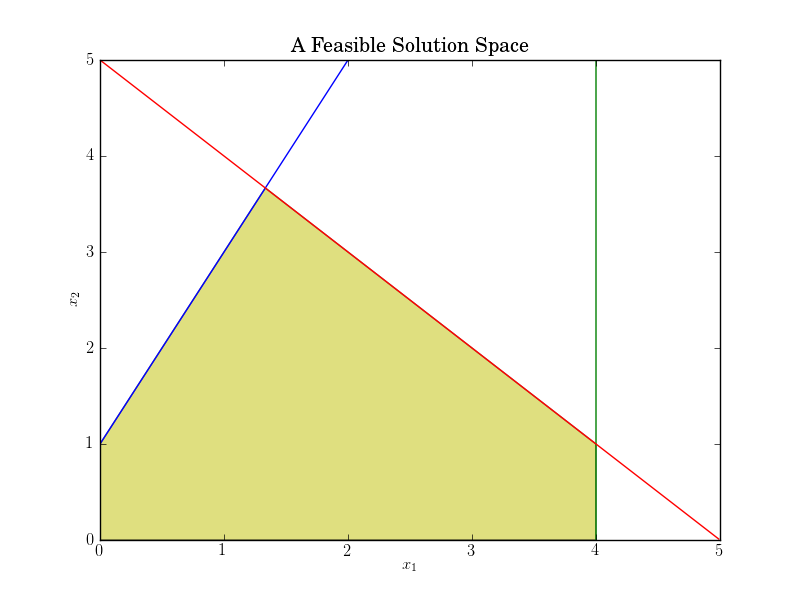
\includegraphics[width=\linewidth]{./chapters/litreview/plots/feasible.png}
  \caption{An example of a feasible solution space.}
  \label{fig:feasible}
  \end{center}
\end{figure}

The program can become infeasible by adjusting a constraint. Take for instance,
an increased boundary constraint for $x_2$.

%%% 
\begin{subequations}\label{eqs:infeas}
  \begin{align}
    %%
    \max \:\: & 
    3 x_1 + 2 x_2
    & \label{eqs:infeas_obj} \\
    %%
    \text{s.t.} \:\: &
    -2 x_1 + x_2 \leq 1 \\
    %%
    &
    x_1 + x_2 \leq 5 
    & \label{eqs:infeas_sup} \\
    %%
    &
    x_1 \in [0, 4]
    &\label{eqs:infeas_x1} \\
    %%
    &
    x_2 \geq 5
    &\label{eqs:infeas_x2}
    %%
  \end{align}
\end{subequations}
%%% 

This arrangement results in the infeasible linear program shown in
Figure \ref{fig:infeasible}, where the updated constraint's effect is shown in
red.

\begin{figure}[H]
  \begin{center}
    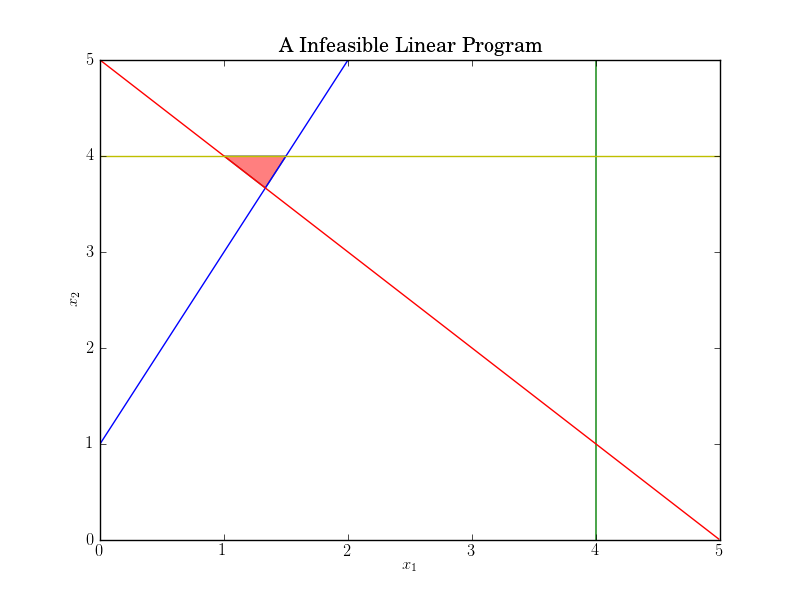
\includegraphics[width=\linewidth]{./chapters/litreview/plots/infeasible.png}
  \caption{An example of a infeasible solution space.}
  \label{fig:infeasible}
  \end{center}
\end{figure}

The standard form of a linear program shown in Equation \ref{eqs:std-form} is an
example of a \textit{primal} linear program. A distinction is made between
a \textit{primal} linear program and its \text{dual}. Duality theory is involved
and only treated lightly in this review. The standard form of the dual of
Equation \ref{eqs:std-form} is given in Equation \ref{eqs:dual-form}.

%%% 
\begin{subequations}\label{eqs:dual-form}
  \begin{align}
    %%
    \max_{u} \:\: & 
    w = b^{\top} u
    & \label{eqs:dual-form_obj} \\
    %%
    \text{s.t.} \:\: &
    A^{\top} u \leq c 
    & \label{eqs:dual-form_sup} \\
    %%
    &
    u \geq 0
    &\label{eqs:dual-form_x}
    %%
  \end{align}
\end{subequations}
%%% 

A few critical differences exist. First note that the objective directions are
switched: if a primal form has a minimization objective, its dual has a
maximization objective. The constraint matrix is now $M$ x $N$-dimensional (it
is in fact the original constraint matrix transposed). There is a new series of
decision variables that form the corresponding solution space, i.e., the
positive vector $u$, as shown in Equation \ref{eqs:dual-form_obj}. These
variables are related to the original right-hand side of the constraint
formulation, the vector $b$. The costs of the original problem, $c$, now form
the right-hand side of the dual's constraint formulation,
Equation \ref{eqs:dual-form_sup}.

The concept of duality is critical in the field of mathematical programming
because it provides well-defined optimality characteristics of a given
program. These are achieved via the \textit{Strong Duality Theorem}
and \textit{Weak Duality Theorem}, shown below as stated
in \cite{ferris_linear_2008}.

\begin{thm}[Weak Duality Theorem]
If $x$ is primal feasible and $u$ is dual feasible, then the dual objective
function evaluated at $u$ is less than or equal to the primal objective function
at $x$.
\end{thm}

The Weak Duality Theorem provides inextricable linkage between a primal feasible
solution and dual feasible solution. If a dual feasible solution is found, it
provides a lower bound on the optimal solution. If a primal feasible solution is
found, it provides an upper bound on the optimal solution. Both of these
criteria, in tandem, help to greatly reduce the required search space during
optimization sweeps.

\begin{thm}[Strong Duality Theorem]
Exactly one of the following three alternatives hold:
\begin{enumerate}

  \item Both primal and dual problems are feasible and consequently both have
  optimal solutions with \textit{equal} extrema

  \item \textit{Exactly one} of the problems is infeasible and consequently the
  other problem has and unbounded objective function in the direction of
  optimization on its feasible region

  \item \textit{Both} primal and dual problems are infeasible

\end{enumerate}
\end{thm}

The Strong Duality Theorem provides the backbone for much of linear programming
theory and application. It states that not only do feasible solutions to the
primal and dual programs provide upper and lower bounds on optimal values, but
that, in fact, the optimal values are \textit{equal}. This provides a criterion
to \textit{know} when an optimal value is reached.

With this slight overview of the realm of linear programming, one can move on to
solution techniques for problems that can be represented as linear programs.
\label{sec:lp-overview}

\subsection{The Simplex Algorithm}\label{sec:simplex}
\subsubsection{Overview}
The Simplex Method is a popular algorithm to solve linear programs first
published by Dantzig \cite{dantzig_maximization_1951}. Conceptually, it is quite
intuitive, especially from a geometrical point of view. I'll introduce the
method first in simple terms to provide a general idea before being a bit more
formal. Let us begin by discussing the example provided in the previous section.

We have the linear program:

%%% 
\begin{subequations}\label{eqs:lp}
  \begin{align}
    %%
    \max \:\: & 
    f(x_1, x_2) = 3 x_1 + 2 x_2
    & \label{eqs:lp_obj} \\
    %%
    \text{s.t.} \:\: &
    -2 x_1 + x_2 \leq 1 \\
    %%
    &
    x_1 + x_2 \leq 5 
    & \label{eqs:lp_sup} \\
    %%
    &
    x_1 \leq 4
    &\label{eqs:lp_x1} \\
    %%
    &
    x_1, x_2 \geq 0
    &\label{eqs:lp_x2}
    %%
  \end{align}
\end{subequations}
%%% 
 
Which appears geometrically as:

\begin{figure}[H]
  \begin{center}
    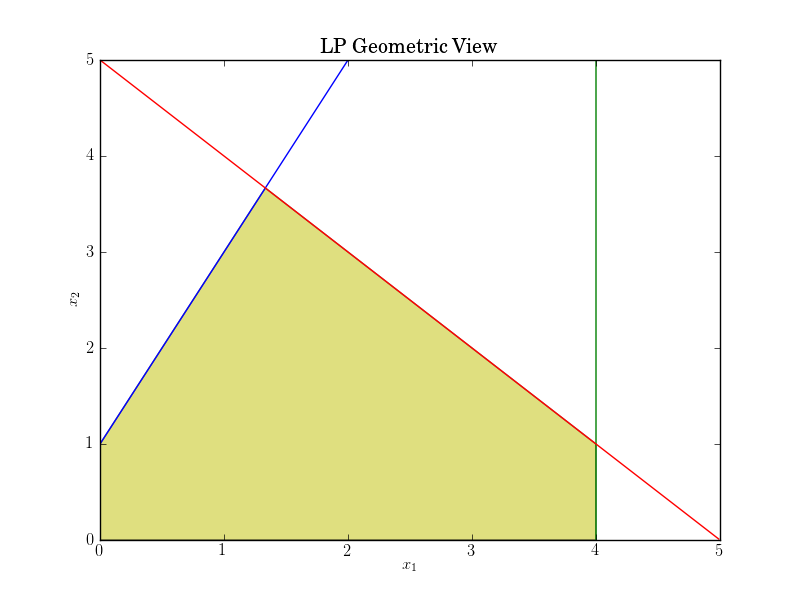
\includegraphics[width=\linewidth]{./chapters/litreview/plots/geometric.png}
  \caption{A Geometric View of the LP.}
  \label{fig:geometric}
  \end{center}
\end{figure}

Note that there are five vertices of the polygon (i.e., polytope) formed by the
full set of constraints:

\begin{enumerate}
  \item $(0, 0)$
  \item $(0, 1)$
  \item $(\frac{4}{3}, \frac{11}{3})$
  \item $(4, 1)$
  \item $(4, 0)$
\end{enumerate}

The Simplex Method begins at a vertex, for example $(0, 0)$, and evaluates the
objective function.

\begin{equation}
    f(0, 0) = 3 * 0 + 2 * 0 = 0 
\end{equation}

Neighbor vertices are then evaluated, in order to determine which provides the
larger value (in the case of maximizing objectives).

\begin{equation}
    f(0, 1) = 3 * 0 + 2 * 1 = 2 
\end{equation}

\begin{equation}
    f(4, 0) = 3 * 4 + 2 * 0 = 12 
\end{equation}

The vertex $(4, 0)$ provides a larger objective function value, so the algorithm
moves to this vertex and determines the next largest neighbor. In this simple
example, there is only one choice, and it is trivially larger.

\begin{equation}
    f(4, 1) = 3 * 4 + 2 * 1 = 14 
\end{equation}

Accordingly the algorithm moves a second time, analyzing the neighboring
vertices again.

\begin{equation}
    f(\frac{4}{3}, \frac{11}{3}) = 3 * \frac{4}{3} + 2 * \frac{11}{3} = \frac{34}{3} 
\end{equation}

At this last move, a terminating condition has been achieved: a vertex has been
found for which all of its neighbors provide a lower value for the objective
function, i.e.,

\begin{equation}
    14 \geq 12 \:\:\: \text{and} \:\:\: 14 \geq \frac{34}{3}.
\end{equation}

Thus, the optimal value for $(x_1, x_2)$ has been determined to be $(4, 1)$. It
is immediately obvious that the simplex algorithm in this state is a hill
climbing (or hill descending) algorithm. The chief reason why this is possible
(i.e., why one is guaranteed to find a globally optimum solution) is that the
objective function and constraints are \textit{convex} functions of the decision
variables. Convexification is a requirement for optimum solutions to both linear
and integer programs, and the tightest possible set of constraints for a given
program describes its \textit{convex hull}.

\subsubsection{In-Depth Discussion}
To begin a more robust discussion of the Simplex Method, one must introduce the
notion of \textit{slack variables}. Slack variables are used to transform
inequality constraints into equality constraints, effectively taking the
``slack'' out of the system. Slack variables are always positive, thus one could
use a slack variable, $s$, to convert

\begin{equation}
  \sum_{i} a_i x_i \leq b
\end{equation}

to 

\begin{equation}
  \sum_{i} a_i x_i + s = b
\end{equation}

and

\begin{equation}
  \sum_{i} a_i x_i \geq b
\end{equation}

to 

\begin{equation}
  \sum_{i} a_i x_i - s = b.
\end{equation}

The addition of slack variables allows one to rewrite an LP given in the
standard form of Equation \ref{eqs:std-form} as the \textit{canonical form}.

%%% 
\begin{subequations}\label{eqs:can-form}
  \begin{align}
    %%
    \min_{x, s} \:\: & 
    z =  c^{\top} x + 0^{\top} s
    & \label{eqs:can-form_obj} \\
    %%
    \text{s.t.} \:\: &
    A x - b = s
    & \label{eqs:can-form_sup} \\
    %%
    &
    x, s \geq 0
    &\label{eqs:can-form_x}
    %%
  \end{align}
\end{subequations}
%%% 

Given that there are $N$ decision variables and $M$ constraints, the cardinality
of $x$ is $N$ and the cardinality of $s$ is $M$. Furthermore, in these examples,
the $x_i$ variables are termed \textit{nonbasic} variables whereas the $s_i$
variables are termed \textit{basic} variables.

For any LP in the canonical form, the Simplex Algorithm can applied to it to
determine optimal values for its decision variables, or to determine that it is
unbounded or infeasible.

\begin{algorithm}[H]
 \SetAlgoLined
 \KwData{Decision variables, an objective function, and a set of constraints.}
 \KwResult{Optimal values for the decision variables or a flag denoting 
   infeasibility or unboundedness.}
 Get initial vertex\;
 \If{no vertex is found}{feasible solution space is empty}
  \While{not unbounded and not empty and not done}{ 
    Select column, i, via pricing\;
    \If{no column is found}{optimal condition found => done}
    Select row, j, via the ratio test\;
    \If{no row is found}{solution space is unbounded}
    Perform a Jordan exchange on element (i, j)\;
  }
  \caption{The Simplex Algorithm}
\end{algorithm}

There are four core operations associated with the Simplex Algorithm:
\begin{enumerate}
  \item finding an initial vertex
  \item column pricing
  \item row selection
  \item exchanging elements
\end{enumerate}

If finding an initial vertex is not trivial (e.g., if the origin is not a
candidate), then the operation to do so requires use of the Simplex Method on a
related LP where the origin is an available candidate. Accordingly, that process
will be described last.

The primary concept required to understand the Simplex Method's operations is
that of the \textit{basis}. The basis begins as the set of decision
variables. The algorithm progresses by moving slack variables into the basis,
and it does so efficiently by analyzing the most ``valuable'' variables to
target (i.e., which current basis variable affects the optimal value the most).

Column pricing and row selection are the operations that select the current
basis and nonbasis variables to target. The Jordan exchange actually performs
the translation of exchanging the basic and nonbasic variables. This is perhaps
more intuitive from a geometrical point of view. Consider some starting vertex
with many possible sides along which to move. The process of column pricing and
row selection \textit{chooses} the side along which to move, and the Jordan
exchange \textit{reorients} the problem. Revisiting the example problem,
remember the first step. The vertex $(4, 0)$ was determined to be the best
direction in which to move. After a Jordan exchange, the resulting LP would look
like Figure \ref{fig:rotated}.

\begin{figure}[H]
  \begin{center}
    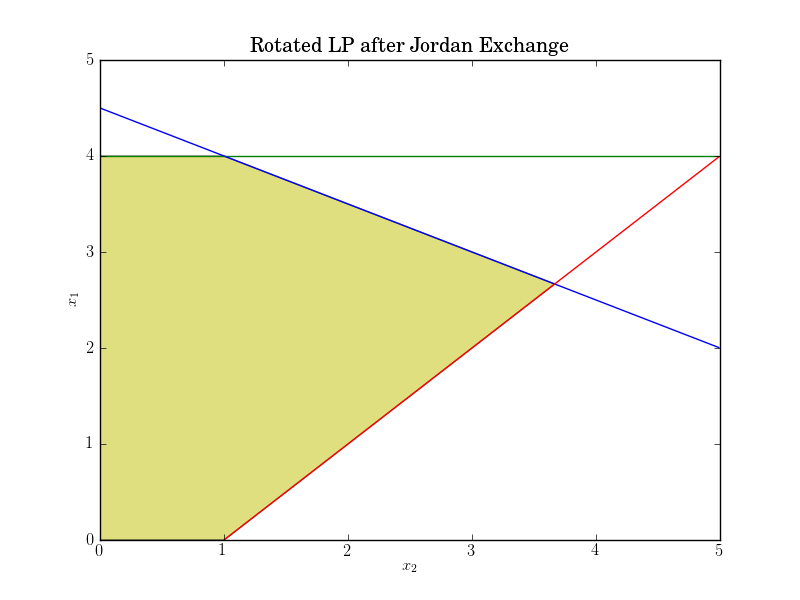
\includegraphics[width=\linewidth]{./chapters/litreview/plots/rotated.png}
  \caption{The Reoriented LP after the first Jordan Exchange.}
  \label{fig:rotated}
  \end{center}
\end{figure}

The column pricing operation selects the slack variable which will enter the
basis. The most naive implementation is to select the variable which will have
the largest effect on the objective function, i.e., which has the largest
magnitude \textit{reduced cost}. For instance, in Equation \ref{eqs:lp_obj},
$x_1$ has a reduced cost of 3, and $x_2$ has a reduced cost of 2 (note that both
costs are in the same positive direction as the objective, i.e.,
maximization). Accordingly, choosing $x_1$ as the nonbasic exchange variable is
a valid option. However, any algorithm may be used to make this selection, as
long as the reduced cost is positive.

Row selection, i.e., selecting the basic variable to enter the basis, is
performed via a ratio test. Given that a column $j$ has been selected, the
corresponding row, and thus basic variable, is selected according to
Equation \ref{eqs:ratio-max} in the case of a maximization objective and
Equation \ref{eqs:ratio-min} in the case of a minimization objective.

\begin{equation}\label{eqs:ratio-max}
  \min \left\{ \frac{-b_i}{A_{i,j}} \:\: | \:\: A_{i,j} > 0 \right\}
\end{equation}

\begin{equation}\label{eqs:ratio-min}
  \min \left\{ \frac{-b_i}{A_{i,j}} \:\: | \:\: A_{i,j} < 0 \right\}
\end{equation}

The Jordan Exchange operation, which transforms a matrix $A \mapsto A'$
given a pivot $(\hat{\imath}, \hat{\jmath})$, is straightforward and is shown in
Equation \ref{eqs:jordan}.

%%% 
\begin{subequations}\label{eqs:jordan}
  \begin{align}
    %%
    a_{\hat{\imath},\hat{\jmath}}' = \frac{1}{a_{\hat{\imath},\hat{\jmath}}}
    &\:\: \text{for} \:
    i = \hat{\imath}, j = \hat{\jmath} \\
    %%
    a_{\hat{\imath},j}' = -\frac{a_{\hat{\imath},j}}{a_{\hat{\imath},\hat{\jmath}}}
    &\:\: \text{for} \:
    i = \hat{\imath}, j \neq \hat{\jmath} \\
    %%
    a_{i,\hat{\jmath}}' = \frac{a_{i,\hat{\jmath}}}{a_{\hat{\imath},\hat{\jmath}}}
    &\:\: \text{for} \:
    i \neq i, j = \hat{\jmath} \\
    %%
    a_{i,j}' = a_{i,j} - a_{i,\hat{\jmath}} a_{\hat{\imath},j}
    &\:\: \text{for} \:
    i \neq \hat{\imath}, j \neq \hat{\jmath}
    %%
  \end{align}
\end{subequations}
%%% 

Finally, one must determine a starting vertex. The original linear program is
modified in the following way. For each row, $i$, if $b_i > 0$, then add an
additional variable, $x_0$ to the constraint with coefficient $a_i,0 = 1$. An
initial feasible point is then immediately available for $x = 0 \forall i \neq
0$ and $x_0 = \max(\max(b),0)$. The Simplex Method is then applied, with $x_0$
being the first variable to leave the basis. When $x_0$ returns to the basis, a
suitable starting vertex results from the removal of $x_0$.


\subsection{Network Flow Problems}\label{sec:xportation}
\subsubsection{Overview}
There are many canonical problems described in the linear programming
literature. A subset of these are classified as network flow programs, which are
ideal for modeling the flows between entities that comprise a model's
formulation. In computational science's parlance, entities make up a set of
nodes in a graph, and the possible connections between those entities make up
the arcs of a graph. Accordingly, if flow can occur between some node $i$ and
some other node $j$, then it flows along arc $(i, j)$. In general there is a set
of nodes $N$ and a set of arcs $A$, as shown in Figure
\ref{fig:node-arcs}. Decision variables in network flow problems determine the
optimal flow between nodes and across arcs.

\begin{figure}[H]
  \begin{center}
    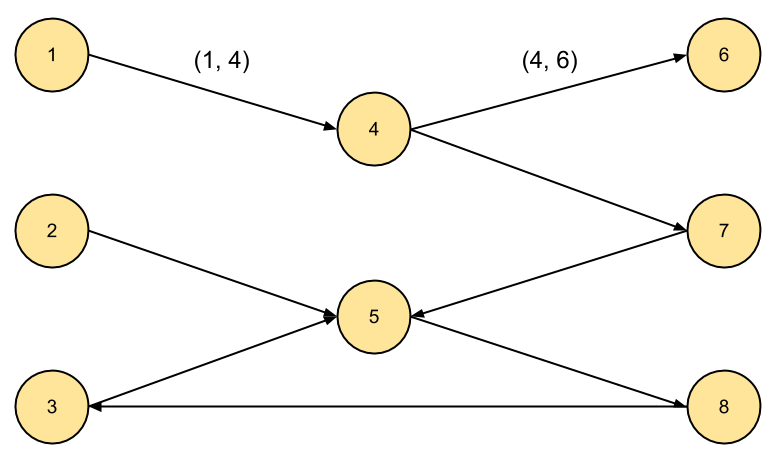
\includegraphics[height=7.5cm]{./chapters/litreview/node-arcs.png}
  \caption{An example node-arc network configuration. Arrows denote possible
    flow directions. Arc notation examples are provided for arcs (1,4) and
    (4,6).}
  \label{fig:node-arcs}
  \end{center}
\end{figure}

The actual formulation for a network flow problem as a linear program is, of
course, dependent on the problem being modeled. Take for example a maximum flow
problem. The objective of such a problem is to maximize the flow in a system,
i.e.,

\begin{equation}
\max \sum_{(i, j) \in A} x_{i,j}.
\end{equation}

The constraint matrix in such problems is denoted a \textit{node-arc incidence}
matrix. For a directed graph, an arc leaving node $i$ and entering arc $j$
indicates a value of 1 for element $a_{i,j}$ and a value of -1 for element
$a_{j,i}$. If an arc between two nodes does not exist, then a value of 0 is
assigned for the two corresponding coefficients. In general network flow
problems, there is also a notion of \textit{divergence}. Divergence is the total
amount of flow exiting or entering a node, and is modeled by the $b$ vector in
the matrix formulation of network flow problems. As is perhaps obvious, if $b_i
> 0$ for some node, $i$, then more flow exits the node than enters it and it is
termed a \textit{source node}. If $b_i < 0$, then more flow enters the node than
flows in, thus it is termed a \textit{sink node}. Finally, if $b_i = 0$, then
all material that flows into the node flows out as well, and it is termed a
\textit{transshipment node}. Finally, arcs can have their flow bounded, where a
lower bound for arc $(i, j)$ is given as $l_{i,j}$ and an upper bound is denoted
$u_{i,j}$.

One can now construct the LP formulation for a max-flow network flow problem.

%%% 
\begin{subequations}\label{eqs:max-flow}
  \begin{align}
    %%
    \max_{x} \:\: & 
    \sum_{(i, j) \in A} x_{i,j}
    & \label{eqs:max-flow_obj} \\
    %%
    \text{s.t.} \:\: &
    \sum_{j:(i,j) \in A} x_{i,j} - \sum_{i:(i,j) \in A} x_{i,j} = b_i
    & \forall i \in N \label{eqs:max-flow_sup} \\
    %%
    &
    l_{i,j} \leq x_{i,j} \leq u_{i,j}
    & \forall (i, j) \in A \label{eqs:max-flow_x}
    %%
  \end{align}
\end{subequations}
%%% 

\subsubsection{Transportation Problems}
Transportation problems are a subset of the network flow problems and can
therefore be modeled using linear programming. Transportation problems model the
flow of a commodity between source nodes and sink nodes, i.e., there are no
transshipment nodes in the general transportation problem. Critically, this
simplification allows for the nodes in the transportation problem to be
categorized into two explicit groups, sources and sinks. In other words, source
nodes and sink nodes comprise two distinct subsets, $N_1, N_2$, the union of
which comprises all nodes in the transportation graph, $N$. These properties can
be described in set notation.

\begin{equation}
  N_1 \subset N
\end{equation}

\begin{equation}
 N_2 \subset N
\end{equation}

\begin{equation}
  N_1 \cup N_2 = N
\end{equation}

From the node-arc graph point of view, this strict subset division allows for
the transportation problem to be modeled as a \textit{bipartite} graph.

\begin{figure}[H]
  \begin{center}
    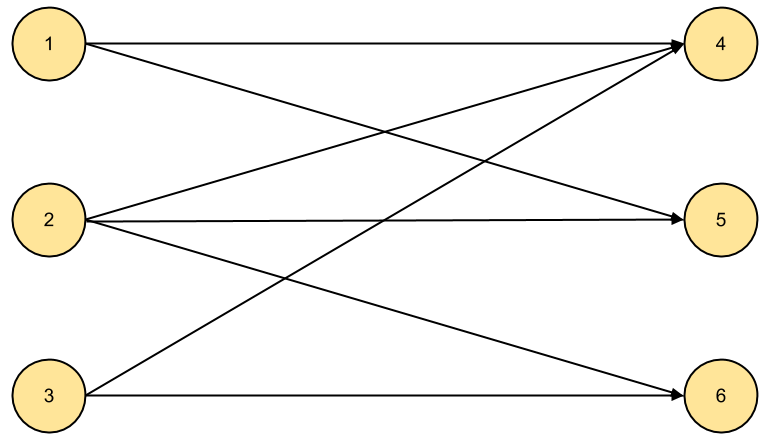
\includegraphics[height=7.5cm]{./chapters/litreview/node-arcs-bipartite.png}
  \caption{An example node-arc transportation network configuration. Arrows
    denote possible flow directions. Note that all nodes either belong to the 
    set of sources (left) or set of sinks (right).}
  \label{fig:node-arcs-bipartite}
  \end{center}
\end{figure}

The transportation problem is a platform on which one can model more general
problems. The minimum-cost transportation problem is a useful example. In such a
formulation, each arc has an associated \textit{unit cost} associated with the
cost of transporting a unit of a commodity along it, $c_{i,j}$. Additionally,
instead of the notion of divergence, supplier and consumer nodes have an
associated supply, $s_i$, or demand, $d_i$, which provide a notion
of \textit{node capacity} rather than arc capacity.

Accordingly, the minimum-cost transportation problem can be formulated as a
linear program in the following manner.

%%% 
\begin{subequations}\label{eqs:xport}
  \begin{align}
    %%
    \min_{x_{i,j}} \:\: & 
    \sum_{(i, j) \in A \subset N_1 \times N_2} c_{i,j} x_{i,j}
    & \label{eqs:xport_obj} \\
    %%
    \text{s.t.} \:\: &
    \sum_{j \in N_2} x_{i,j} \leq s_i
    & \forall i \in N_1  \\
    %%
    &
    \sum_{i \in N_1} x_{i,j} \geq d_i
    & \forall j \in N_2  \\
    %%
    &
    x_{i,j} \geq 0
    & \forall i \in N_1, \: \forall j \in N_2 \label{eqs:xport_x}
    %%
  \end{align}
\end{subequations}
%%% 

As is noted in many texts on the Transportation Problem Linear Program
formulation, an intuitive constraint on the problem to guarantee a feasible
solution is that the total demand in the system must be no greater than the
total supply in the system.

\begin{equation}
  \sum_{j \in N_2} d_j \leq \sum_{i \in N_1} s_i
\end{equation}

Feasibility in this sense can be guaranteed, however, by adding an artificial
supply node. Such a node can have infinite supply capacity but at (effectively)
infinite cost. The problem can then be solved, and any flow leaving the
artificial node in the optimal solution can be dealt with accordingly, e.g., it
can be ignored.

\subsubsection{Multi-Commodity Transportation Problems}\label{sec:MCTP}
The previously-described transportation problem can more precisely be named the
single-commodity transportation problem. It deals with the flow from sources to
sinks of a single commodity. A more complex model includes more than one
commodity.

Variables and constants in the multi-commodity formulation are generally analogs
of their counterparts in the single-commodity problem. There is a unit cost for
commodity $h$ to traverse arc $(i,j)$ denoted as $c_{i,j}^{h}$. A supplier of
commodity $h$ has a certain supply capacity $s_i^h$ which cannot be surpassed
and demanders of commodity $h$ have a certain demand level which must be met,
$d_i^h$.

In the simplest extension from the single-commodity to multi-commodity
transportation problem, arc constraints for all commodities are combined, i.e.,
for a given arc $(i, j)$, there is a single capacity $u_{i,j}$. A classic
interpretation of this enhanced complexity deals with data networks. Multiple
classifications of data exist, but they all must traverse the same network
infrastructure. Accordingly, the infrastructure can only accommodate a certain
level of total flow among all communication types.

This coupling of commodities via arc capacities changes the structure of the
node-arc incidence matrix. Arc capacity constraints no longer have a single
entry. Instead, many flows contribute to the capacity constraint, requiring
different methods to solve the problem. Of course, the Simplex Method can still
solve the linear program, however other potential reductions in time and
complexity that are available to the single-commodity flow problem are not
available to the multi-commodity flow problem due to this coupling.

The formulation of the multi-commodity flow problem is shown in Equation
\ref{eqs:MCTP}. Note the commodity coupling in Equation \ref{eqs:MCTP_cap}.

%%% 
\begin{subequations}\label{eqs:MCTP}
  \begin{align}
    %%
    \min_{x_{i,j}^{h}} \:\: & 
    \sum_{i \in I}\sum_{j \in J}\sum_{h \in H} c_{i,j}^{h} x_{i,j}^{h}
    & \label{eqs:MCTP_obj} \\
    %%
    \text{s.t.} \:\: &
    \sum_{j \in J} x_{i,j}^{h} \leq s_{i}^{h}
    &
    \forall \: i \in I, \forall \: h \in H \label{eqs:MCTP_sup} \\
    %%
    &
    \sum_{i \in I} x_{i,j}^{h} \geq d_{j}^{h}
    & 
    \forall \: j \in J, \forall \: h \in H \label{eqs:MCTP_dem} \\
    %%
    &
    \sum_{h \in H} x_{i,j}^{h} \leq u_{i,j}
    & 
    \forall \: j \in J \label{eqs:MCTP_cap} \\
    %%
    &
    x_{i,j}^{k} \geq 0
    &
    \forall \: i \in I, \forall \: j \in J, \forall \: h \in H \label{eqs:MCTP_x}
    %%
  \end{align}
\end{subequations}
%%% 

A number of important reductions are possible for the multi-commodity
transportation problem, e.g., the case in which is no arc that shares multiple
commodities. In this instance the multicommodity connection constraints
disappear, and the single multi-commodity problem can be broken into $m$
different single-commodity transportation problems, where $m$ is the cardinality
of the set of commodities, $H$. 


\subsection{Linear Approximation Problems}\label{sec:approx}
Another application of linear programming involves approximating solutions to
linear systems of equations in the form of Equation \ref{eqs:lin-sys}.

\begin{equation}\label{eqs:lin-sys}
A x = b
\end{equation}

$A$ is an $m x n$-dimensional constraint matrix that can
be \textit{overdetermined}, i.e., include more constraints than decision
variables. Given some approximation of the solution, $\tilde{x}$, one can define
the residual, $r$, associated with that approximation.

\begin{equation}\label{eqs:lin-sys}
A \tilde{x} - b = r
\end{equation}

One can then formulate an optimization problem that seeks to minimize the
$\ell_p$-norm of the residual vector, $r$. The literature treats three types of
norms, $\ell_1$, $\ell_2$, and $\ell_\infty$, where each can be defined as
follows.

\begin{equation}
\ell_1 (r) = \| r \|_1 = \sum_{i = 1}^{m} | r_i |
\end{equation}

\begin{equation}
\ell_2 (r) = \| r \|_2 = \sqrt{ \sum_{i = 1}^{m} | r_i |^2 }
\end{equation}

\begin{equation}
\ell_\infty (r) = \| r \|_\infty = \max_{i} | r_i |
\end{equation}

The linear programming formulation takes as its minimizing function the
residual, for which individual $x_i$ values form the decision
variables. Accordingly, each $\ell_p$ norm formulation is slightly
different. 

The $\ell_\infty$ norm utilizes a maximum-violation variable $\epsilon$, as shown
in Equation \ref{eqs:l-inf}.

%%% 
\begin{subequations}\label{eqs:l-inf}
  \begin{align}
    %%
    \min \:\: & 
    \epsilon  \\
    %%
    \text{s.t.} \:\: &
    - \epsilon \leq A_i x - b_i
    & \forall i \\
    %%
    &
    \epsilon \geq A_i x - b_i
    & \forall i \\
    %%
  \end{align}
\end{subequations}
%%% 

The $\ell_1$ norm uses a summation over all violations, as shown in
Equation \ref{eqs:l-1}, by using a proxy vector, $y$.

%%% 
\begin{subequations}\label{eqs:l-1}
  \begin{align}
    %%
    \min \:\: & 
    \sum_i y
    & \\
    %%
    \text{s.t.} \:\: &
    - y_i \leq A_i x - b_i
    & \forall i \\
    %%
    &
    y_i \geq A_i x - b_i
    & \forall i \\
    %%
  \end{align}
\end{subequations}
%%% 

The core difference between the two formulations is of course the norm used. The
$\ell_1$ norm in this case stores more information about the total violation,
whereas the $\ell_\infty$ norm is concerned with only the largest violating
constraint. These formulations are easily solved by the Simplex Method, as a
starting vertex can always be chosen by setting $x = 0$.

The $\ell_2$ norm is not as straightforward to solve. As shown
in \ref{ferris_linear_2008}, the actual norm can be replaced by its square,
because it is uniformly nonnegative. The resulting optimization problem is shown
in Equation \ref{eqs:l-2}.

%%% 
\begin{subequations}\label{eqs:l-2}
  \begin{align}
    %%
    \min \:\: & 
    y^\top y
    & \\
    %%
    \text{s.t.} \:\: &
    - y_i \leq A_i x - b_i
    & \forall i \\
    %%
    &
    y_i \geq A_i x - b_i
    & \forall i \\
    %%
  \end{align}
\end{subequations}
%%% 

As can be seen in its formulation in Equation \ref{eqs:l-2}, the objective
function is not a linear function of the decision variables. Accordingly, one
must tackle this problem using a different domain of mathematical programming,
namely \textit{quadratic programming}, the discussion of which is outside the
scope of this review due to the lack of its necessity to adequately solve the
Recipe Approximation Problem described in \S\ref{sec:rap}.


\section{Integer Programming}\label{sec:ip}
Integer programming expands upon the possible problems that can be modeled by
linear programming. Decision variables in linear programming are optimized on a
continuum, i.e., all decision variables, $x$, are real numbers,
$x \in \mathbb{R}^n$. Integer programming allows for certain decision variables,
$y$, to take on integer-only values, i.e., $y \in \mathbb{Z}^n$. Strictly
speaking, a programming formulation for which all decision variables are integer
(i.e., integer and binary) is called an \textit{integer program} (IP), whereas a
programming formulation for which some decision variables are integer while
others are linear is called a \textit{mixed integer-linear program} (MILP). The
discussion that follows is informed largely by Wolsey's
text \cite{wolsey_integer_1998} from which I cite many definitions,
etc. Additional clarification comes from course notes \cite{luedtke_class_2010}.

Integer programming allows one to model specialized decision cases. Take for
example one of the most well-known problems in mathematical programming and
optimization, the \textit{Knapsack Problem}. A version of the Knapsack problem
is described as follows:

\begin{itemize}
        \item A knapsack can hold at most $b$ pounds. 
        \item There are $n$ possible items that can be placed in the bag.
        \item Each item is characterized by a preference, or benefit, $c_i$, 
              and a weight, $a_i$
        \item One would like to maximize the benefit associated with a knapsack
\end{itemize}

The decision variables, $y_i$s, for the Knapsack Problem provide its integer
nature. Any given item in the above formulation can only be added once. Indeed,
consider that for any viable solution, each item is in one of two distinct
states: included in the knapsack or excluded from the knapsack. This duality of
states provides a natural usage of binary variables, i.e., a variable that has
only two states, 0 and 1. Accordingly, the Knapsack Problem as an integer
program is formulated as Equation \ref{eqs:knapsack}.

%%% 
\begin{subequations}\label{eqs:knapsack}
  \begin{align}
    %%
    \max \:\: & 
    \sum_{i \in I} c_i y_i
    & \\
    %%
    \text{s.t.} \:\: &
    \sum_{i \in I} a_i y_i \leq b 
    & \\
    %%
    &
    y_i \in \{ 0, 1 \}
    &
    \forall i \in I
    %%
  \end{align}
\end{subequations}
%%% 

\subsection{Computational Complexity}\label{sec:complexity}

In general, optimization problems are solved by solving a number of decision
problems. Decision problems are generally
computationally \textit{hard}. Decision problems ask yes or no questions,
e.g., ``is there a knapsack packing that with a benefit higher than $x$?''. An
optimization problem asks instead ``what is the knapsack packing with the
highest benefit?''. Any problem can be associated with one of four categories of
computational complexity:

\begin{itemize}
        \item Polynomial-time ($\mathcal{P}$)
        \item Nondeterministic Polynomial-time ($\mathcal{NP}$)
        \item Nondeterministic Polynomial-time Complete  ($\mathcal{NP}$-C)
        \item Nondeterministic Polynomial-time Hard  ($\mathcal{NP}$-hard)
\end{itemize}

The topic of computational complexity is relatively involved, thus I will only
provide a short overview to provide context. A problem is considered to reside
in $\mathcal{P}$ if there is a polynomial-time algorithm that can solve it. A
classic example is that of naive matrix inversion, known to be of order $n^3$
(i.e., $\mathcal{O}(n^3)$) for a given $n \times n$ matrix.

A decision problem is considered to be in ($\mathcal{NP}$) if for any proposed
solution, there is a \textit{short certificate}.

\begin{define}
A \textbf{certificate} is a method to verify that a solutions provides a
positive or negative response to the question at hand. A certificate is
considered \textbf{short} if it is polynomial in size and can be verified in
polynomial time.
\end{define}

A decision problem, $Q$, is considered to be in $\mathcal{NP}$-C, if
$Q \in \mathcal{NP}$ and \textit{any} problem, $P \in \mathcal{NP}$ is
polynomial-time reducible to $Q$, i.e., instances of $P$ can be reformulated as
instances of $Q$ in polynomial time. The most popular candidate of this
polynomial reduction is the Satisfiability Problem, known to be in
$\mathcal{NP}$-C.

Finally, a problem $Q$, is in $\mathcal{NP}$-hard, if any problem
$P \in \mathcal{NP}$ is polynomial-time reducible to $Q$, but
$Q \not\in \mathcal{NP}$. If a decision problem is in $\mathcal{NP}$-C, then the
corresponding optimization problem is $\mathcal{NP}$-hard.

The various levels of complexity are related. It is not known whether
$\mathcal{P} = \mathcal{NP}$, but it is strongly suspected that
$\mathcal{P} \subset \mathcal{NP}$. It is also assumed that
$\mathcal{NP}\text{-C} \subset \mathcal{NP}$, and
$\mathcal{NP}\text{-hard} \notin \mathcal{NP}$ by definition. The relationship
between these set of problem complexities is shown graphically in
Figure \ref{fig:complexity}.

\begin{figure}[H]
  \begin{center}
    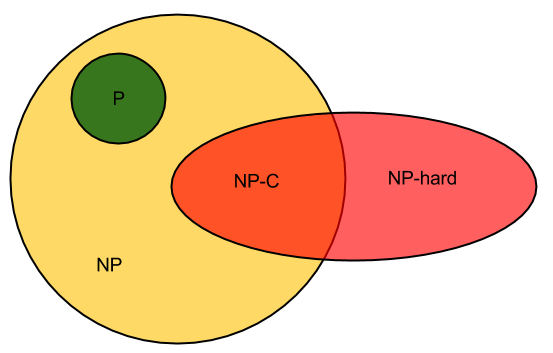
\includegraphics[height=7.5cm]{./chapters/litreview/complexity.png}
  \caption{The relationship between the various types of problem complexities.}
  \label{fig:complexity}
  \end{center}
\end{figure}


\subsection{Formulations and Cutting Planes}\label{sec:formulations}

Optimization problems are given as formulations, a series of inequality
equations. Both domain knowledge and geometrical investigation can provide
better formulations than may be evident from an initial formulation. Formally, a
formulation forms a polyhedron.

\begin{define}\label{def:polyhedron}
A subset of $\mathbb{R}^n$ described by a finite set of linear constraints $P
= \{ x \in \mathbb{R}^n : Ax \leq b\}$ is a \textbf{polyhedron}.
\end{define}

\begin{define}\label{def:formulation}
A polyhedron $P \subseteq \mathbb{R}^{n+p}$ is a \textbf{formulation} for a set
$X \subseteq \mathbb{Z}^n \times \mathbb{R}^p$ iff $X = P \cap \left( 
\mathbb{Z}^n \times \mathbb{R}^p \right)$
\end{define}

As previously noted, more than one formulation can be viable for a given
problem. Let us return to the Knapsack Problem in
Equation \ref{eqs:knapsack}. Consider a knapsack with $b = 5$ and items with
$a_1 = 2$, $a_2 = 3$, $a_3 = 4$. The original formulation is as follows.

%%% 
\begin{subequations}\label{eqs:knapsack1}
  \begin{align}
    %%
    \max \:\: & 
    \sum_{i \in I} c_i y_i
    & \\
    %%
    \text{s.t.} \:\: &
    2y_1 + 3y_2 + 4y_3 \leq 5 
    & \\
    %%
    &
    y_i \in \{ 0, 1 \}
    &
    \forall i \in I
    %%
  \end{align}
\end{subequations}
%%% 

The set of feasible solutions here forms a polyhedron from the points $Y = {(0,
0, 0), (1, 0, 0), (0, 1, 0), (0, 0, 1), (1, 1, 0)}$. The optimal solution will
depend on values given to each item's benefit, $c_i$. However, the formulation
as provided defines a solution space larger than the specific points mentioned
here. One could add a constraint, say, 

\begin{equation}
y_1 + y_3 \leq 1
\end{equation}

or 

\begin{equation}
y_2 + y_3 \leq 1.
\end{equation}

These two constraints state that the third item, if chosen, can not be included
with either the first or the second item. The resulting formulation is shown in
Equation \ref{eqs:knapsack2}.

%%% 
\begin{subequations}\label{eqs:knapsack2}
  \begin{align}
    %%
    \max \:\: & 
    \sum_{i \in I} c_i y_i
    & \\
    %%
    \text{s.t.} \:\: &
    2y_1 + 3y_2 + 4y_3 \leq 5 
    & \\
    %%
    &
    y_1 + y_3 \leq 1        
    & \\
    %%
    &
    y_2 + y_3 \leq 1        
    & \\
    %%
    &
    y_i \in \{ 0, 1 \}
    &
    \forall i \in I
    %%
  \end{align}
\end{subequations}
%%% 

It is obvious that Equation \ref{eqs:knapsack2} is a different formulation than
Equation \ref{eqs:knapsack1}. For example, the point $(0.9, 0.5, 0.4)$ resides
in the feasible solution space of Equation \ref{eqs:knapsack1} but is outside of
the feasible solution space of Equation \ref{eqs:knapsack2}. Intuitively, a
smaller solution space can be searched more quickly, thus \textit{tighter}
formulations require less time to solve in general.

The notion of one formulation being ``better'' than another can be formally
expressed.

\begin{define}
Given a set $X \subseteq \mathbb{R}^n$ and two formulations, $P_1$ and $P_2$,
for $X$, $P_1$ is a \textbf{better formulation} than $P_2$ if $P_1 \subset P_2$.
\end{define}

There is, of course, a limit to the formulations one can develop for a given
problem. A fully-restricted solution space, i.e., one that is as tightly bounded
as possible, is called the problem's \textit{convex hull}. 

\begin{define}
Given a set $X \subseteq \mathbb{R}^n$, the \textbf{convex hull} of $X$, denoted
$conv(X)$, is defined as: $conv(X) = \{x : x = \sum_{i=1}^{t} \lambda_i
x_i, \sum_{i=1}^{t} \lambda_i = 1, \lambda_i \geq 0$ for $i = 1, \ldots, t$ over
all finite subsets $\{x^1, \ldots, x^t \}$ of $X\}$.
\end{define}

Because the extreme points of $conv(X)$ all lie in $X$, the equivalent LP can be
used instead of the IP. Convex hull formulations are rarely seen in practice,
however, because they require an exponential number of additional
constraints \cite{wolsey_integer_1998}. While the convex hull of a given problem
may not be discovered in practice, the feasible solution space most assuredly is
reduced by most solution techniques. From a geometrical point of view, this acts
as cutting off solution space from some original larger space through the
addition of constraints as shown above. Accordingly, these additional
constraints are termed \textit{cutting planes}.

\subsection{The Branch and Bound Algorithm}\label{sec:bnb}

One of the most popular solution techniques used to solve integer programs is an
algorithm called \textit{Branch and Bound} (BNB). At its core, BNB is a
divide-and-conquer search algorithm that uses an enumeration tree to find
optimal solutions to $\mathcal{NP}$-hard IPs and MILPs. There are a number of
ways to speed up the search based on general techniques and problem-specific
insights, a number of which have been discussed in the previous section. This
section highlights the basic nature of the algorithm and discusses lightly some
of the variety of solution strategies available. Again, the discussion here
comes largely from \cite{wolsey_integer_1998} and \cite{luedtke_class_2010}.

BNB utilizes the \textit{relaxation} of a given IP or MILP. A relaxation is a
related reformulation of a given problem that is generally easier to solve. In
the case of a linear programming relaxation, integer variables in the IP or MILP
are relaxed and allowed to be linear variables. Solving this formulation is
advantageous because it provides an \textit{upper bound} for the IP or
MILP. Similarly, solving a dual, given that it is feasible and has a finite
solution, or using some other heuristic provides a \textit{lower bound}. These
bounds allow the search tree to terminate, or \textit{prune}, a
given \textit{branch}.

A simple example greatly helps to show the process of the BNB algorithm. Let us
use a specific instance of Equation \ref{eqs:knapsack}. This example is
contrite and does not involve pruning; it is useful simply to show how
branching occurs. Consider a knapsack with three items. The items have benefits
of 0.5, 1, and 1.4, respectively and weights of 2, 3, and 4 pounds,
respectively. The knapsack can hold 5 pounds. The integer program is shown in
Equation \ref{eqs:knapsack-ip} and the LP relaxation is shown in
Equation \ref{eqs:knapsack-lp}.

%%% 
\begin{subequations}\label{eqs:knapsack-ip}
  \begin{align}
    %%
    \max \:\: & 
    Z^{IP} = 0.5 y_1 + y_2 + 1.4 y_3
    & \\
    %%
    \text{s.t.} \:\: &
    2y_1 + 3y_2 + 4y_3 \leq 5 
    & \\
    %%
    &
    y_1, y_2, y_3 \in \{ 0, 1 \}
    %%
  \end{align}
\end{subequations}
%%% 

%%% 
\begin{subequations}\label{eqs:knapsack-lp}
  \begin{align}
    %%
    \max \:\: & 
    Z^{LP} = 0.5 y_1 + y_2 + 1.4 y_3
    & \\
    %%
    \text{s.t.} \:\: &
    2y_1 + 3y_2 + 4y_3 \leq 5 
    & \\
    %%
    &
    y_1, y_2, y_3 \in [0, 1]
    %%
  \end{align}
\end{subequations}
%%% 

Solving the relaxation provides an upper bound of $Z^{LP} = \frac{26}{15}$, a
(non-integer) solution of $y' = (0, \frac{1}{3}, 1)$ and a root node for the BNB
search tree, shown in Figure \ref{fig:root}.

\begin{figure}[H]
  \begin{center}
    
\includegraphics[width=0.8\linewidth]{./chapters/litreview/root.png}
  \caption{The root node for the BNB algorithm associated with 
  Equation \ref{eqs:knapsack-ip}.}
  \label{fig:root}
  \end{center}
\end{figure}

The algorithm then chooses a variable on which to \textit{branch}. Formally
branching divides the set of feasible solution spaces in two. Given a solution
space $S$, branching on a binary variable $y_i$, produces two new solution
spaces.

\begin{equation}
\begin{split}
& S_1 = S \cap \{y: y_i = 0\}
\\
& S_2 = S \cap \{y: y_i = 1\}
\end{split}
\end{equation}

If the variable is non-binary integer, given a non-integer feasible solution,
$y'$, one produces the following new spaces.

\begin{equation}
\begin{split}
& S_1 = S \cap \{y: y_i \leq \lfloor y_i' \rfloor\}
\\
& S_2 = S \cap \{y: y_i \geq \lceil y_i' \rceil\}
\end{split}
\end{equation}

Arbitrarily, for this example case, one could choose to branch on
$y_2$. The resulting relaxations are shown as Equation \ref{eqs:y2-0} for $y_2 =
0$ and Equation \ref{eqs:y2-1} for $y_2 = 1$.

%%% 
\begin{subequations}\label{eqs:y2-0}
  \begin{align}
    %%
    \max \:\: & 
    Z^{LP} = 0.5 y_1 + 1.4 y_3
    & \\
    %%
    \text{s.t.} \:\: &
    2 y_1 + 4 y_3 \leq 5 
    & \\
    %%
    &
    y_1, y_3 \in [0, 1]
    %%
  \end{align}
\end{subequations}
%%% 

%%% 
\begin{subequations}\label{eqs:y2-1}
  \begin{align}
    %%
    \max \:\: & 
    Z^{LP} = 0.5 y_1 + 1 + 1.4 y_3
    & \\
    %%
    \text{s.t.} \:\: &
    2 y_1 + 3 + 4 y_3 \leq 5 
    & \\
    %%
    &
    y_1, y_3 \in [0, 1]
    %%
  \end{align}
\end{subequations}
%%% 

Each of these new subproblems become \textit{active nodes} and are added to
the \textit{active list}. Active nodes are subproblem nodes that have been
recognized by the algorithm and the next subproblem to solve is chosen from the
active list by some strategy. For this simple case, both subproblems are solved
and the resulting values are shown in Figure \ref{fig:branch}.

\begin{figure}[H]
  \begin{center}
    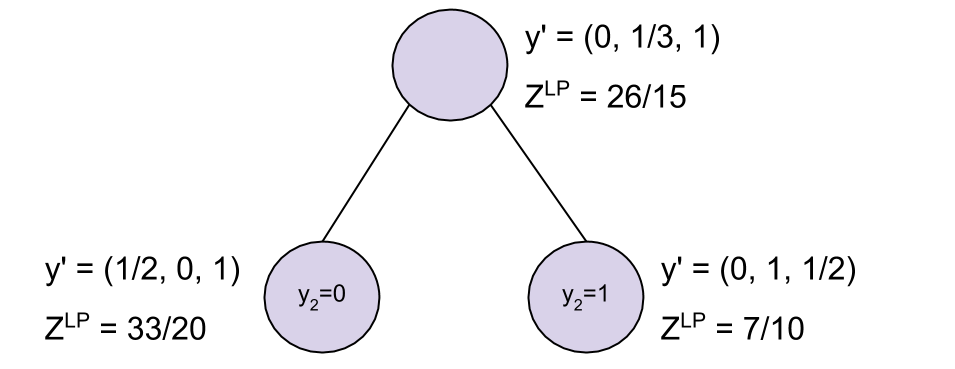
\includegraphics[height=5.5cm]{./chapters/litreview/branch.png}
  \caption{The first two branches of the BNB algorithm associated with 
  Equations \ref{eqs:y2-0} and \ref{eqs:y2-1}.}
  \label{fig:branch}
  \end{center}
\end{figure}

One could continue in this manner, branching on subsequent variables and
enumerating all possible solutions, to eventually reach the optimal solution of
$y^* = (1, 1, 0)$. However, so far we have ignored pruning, the act of
terminating a branch of the search tree, knowing that no further useful
information can be gained from its investigation. Pruning provides the
``bounding'' aspect of the Branch and Bound algorithm.

At any point in the process of the BNB algorithm, there is a known global upper
bound, $U$, to the optimal solution and lower bound, $L$, to the optimal
solution. Accordingly, a branch of the enumeration search tree can be pruned in
three instances:

\begin{enumerate}
        \item The subproblem is optimal, given its subspace of the feasible
        option space.
        \item The subproblem has a known upper bound that is lower
        than the global lower bound or the subproblem has a known lower bound
        that is larger than the global upper bound.
        \item The subproblem is infeasible.
\end{enumerate}

With the above background, the actual BNB algorithm can be presented.
\\
\begin{algorithm}[H]
 \SetAlgoLined
 \KwData{Decision variables, an objective function, and a set of constraints.}
 \KwResult{Optimal values for the decision variables or a flag denoting 
   infeasibility or unboundedness.}
 Perform any \emph{preprocessing operations}\;
 Derive a lower bound, $L$, via a \emph{heuristic}\;
 Place original problem on the active list\;
 \While{The active list is \textit{not} empty}{
       Use a \emph{strategy} to select a candidate node ($S$) from the active 
       list\;
       Solve the LP relaxation to get an upper bound for the candidate, $U(S)$\;
       \If{$U(S) > U$}{$U \leftarrow U(S)$\;}
       \If{$S$ is infeasible}{
           prune the branch\;
       }
       \ElseIf{$U(S) > L$}{
           $L \leftarrow U(S)$\;
       }
       \ElseIf{$U(S) < L$}{
           prune the branch\;
       }
       \Else{
           branch on $S$\;
           add new subproblems to the active list\;
       }           
       Remove $S$ from the active list\;
 }
 \caption{The Branch and Bound Algorithm}
\end{algorithm}

There are three ways to assist, or speed up, the Branch and Bound algorithm as
highlighted above:
\begin{enumerate}
        \item Preprocessing
        \item Lower-bound heuristics
        \item Node selection strategies
\end{enumerate}

Preprocessing is a step provided by many solvers. It generally involves an
investigation of the problem instance in order to minimize future
work. Preprocessing can affect solution bounds by tightening bounds or providing
cutoffs to the solver (i.e., preformed feasible solutions). It can speed up the
internal Simplex Method processing by informing the solver as to good simplex
pricing strategies. The feasible solution space can also be reduced by finding
redundant constraints and providing cutting planes, as discussed in the previous
section. Finally, the preprocessing step can \textit{a priori} fix certain
decision variables. The variable fixing algorithm is straightforward.

\begin{algorithm}[H]
 \SetAlgoLined
 \KwData{An constraint matrix, $A$, objective coefficients, $c$, and decision 
 variables $x$ with decision variable lower bounds, $l$, and upper bounds 
 $u$.}
 \KwResult{A (possibly empty) set of fixed variables.}
 \ForEach{decision variable, $x_j$,}{
   \If{$a_{i,j} \geq 0 \;\; \forall \;\; i$ {\emph{and}} $c_j < 0$}{
     $x_j \leftarrow l_j$\;
   }
   \ElseIf{$a_{i,j} \leq 0 \;\; \forall \;\; i$ {\emph{and}} $c_j > 0$}{
     $x_j \leftarrow u_j$\;
   }       
 }  
 \caption{The Variable Fixing Algorithm for a Maximization Objective Function}
\end{algorithm}

A variety of lower-bound heuristics exist. Some of the most popular involve
solving heavily restricted versions of the original problem or diving down the
enumeration tree, rounding fractional integer values. There are also
problem-specific heuristics that depend on well-known problem structures.

Finally, there exist nominally three well-used node selection strategies. The
first is called the \textit{Best Node Search} (BNS) which chooses the next best
node in the active list based based on the node's upper bound. This requires
large movement around the search tree, effectively solving dissimilar
relaxations. The second is the well-known \textit{Depth First Search} (DFS). A
DFS for an IP-enumeration tree is beneficial because subsequent relaxations are
related, which allows for \textit{warm start} of the LP relaxations. Warm starts
allow subsequent relaxations to be solved quickly because good approximations to
the optimal solution can be provided. The final strategy is a \textit{BNS-DFS
hybrid}. The hybrid strategy involves estimating an optimal value, performing a
DFS until the relaxation's optimal value is below that of the estimation, and
then choosing the next-best node to continue.

